%%%%% 
% 
% WORKFLOW MODUL TINF13AIBC
% S. Wagner, M. Doerfler, J. Dann / SAP AG, Juni 2014
%
%%%%%

\documentclass[12pt,pdftex,a4paper,oneside,ngerman]{scrreprt}

% Settings of TeX Document
%%%
%
% haeufig benoetigte Festlegungen
%
%%%

%% Erweiterungspakete werden geladen

% erlaubt direkte Verwendung von Umlauten im Quelltext (latin1)
%\usepackage{umlaut} 
\usepackage[utf8]{inputenc}% http://ctan.org/pkg/inputenc

% länderspezifische Einstellungen
% sorgt u.a. für die korrekte Silbentrennung,
% deutsche Bezeichner ("Tabelle", "Abbildung" etc.)
\usepackage[ngerman]{babel}

% fuer deutsche W"orter in der Literaturliste
\usepackage{bibgerm}  

% Sonderzeichen, z.B. Euro mit \texteuro   
\usepackage{textcomp}         

% erlaubt einfache Auswahl der Art der Nummerierung bei Aufzählungen
\usepackage{enumerate}

% erlaubt das Einbinden von Grafiken
\usepackage{graphicx}

% erlaubt die einfache Aenderung der Seitenraennder
%\usepackage[left=15mm,right=15mm,top=19mm,bottom=19mm]{geometry}

\usepackage[ngerman]{translator}

\usepackage{tabularx}    
                       
\usepackage{booktabs}  

\usepackage{setspace} 

\usepackage{amssymb}

\usepackage{eurosym}

\usepackage{lastpage}

\usepackage{multicol}

\usepackage{pgf-pie,etoolbox}

\usepackage{wrapfig}

\usepackage{float}

\definecolor{light-gray}{gray}{0.95}

% ------------------------------ Listings --------------------------------------

\usepackage{listings}

\lstdefinelanguage{HANASQL}
{
morestring=[b]",
morestring=[s]{>}{<},
morecomment=[s]{<?}{?>},
stringstyle=\color{black},
identifierstyle=\color{darkblue},
keywordstyle=\color{cyan},
morekeywords={CREATE, INSERT},% list your attributes here
backgroundcolor=\color{light-gray}, % Hintergrundfarbe des Quellcodes setzen.
captionpos=b,
breakautoindent=true, 
}

\lstset{numbers=left, 
				numberstyle=\tiny, 
				breaklines=true,
				backgroundcolor=\color{light-gray},
				numbersep=5pt,
				xleftmargin=.25in,
				xrightmargin=.25in,
				captionpos=b,
				basicstyle=\ttfamily,
				keywordstyle=\color{blue}\ttfamily,
				stringstyle=\color{red}\ttfamily,
				commentstyle=\color{green}\ttfamily,
}

% ------------------------------ Geometrie--------------------------------------
\usepackage{geometry,blindtext}
\geometry{a4paper,left=30mm,right=20mm, top=1cm, bottom=2cm, includeheadfoot}

% ---------------------------- Kopf-Fußzeilen-----------------------------------
\usepackage{fancyhdr}
\pagestyle{fancy}
\fancyhf{}

\fancyhead[L]{\small{\textbf{Proseminar Workflow}}}
\fancyhead[C]{\chaptername~\thechapter}
\fancyhead[R]{
\includegraphics[scale=0.1]{grafiken/sap_logo.png}}
\renewcommand{\headrulewidth}{0.5pt} %obere Trennlinie
\fancyfoot[C]{\thepage\ von \pageref{LastPage}} %Seitennummer
\renewcommand{\footrulewidth}{0.4pt} %untere Trennlinie
\def\chapterpagestyle{fancy} %auch bei Seiten mit Chapter Kopfzeile anzeigen
%\addtocontents{toc}{\protect\thispagestyle{fancy}} %nicht auf Inhaltsverzeichnis
\addtocontents{toc}{\protect\thispagestyle{empty}}
\addtocontents{lof}{\protect\thispagestyle{empty}}
\addtocontents{lot}{\protect\thispagestyle{empty}}
\addtocontents{lol}{\protect\thispagestyle{empty}}

% ----------------------------- Hyperlinks -------------------------------------
\usepackage{breakurl}         % Zeilenumbruch f"ur URLs

% Links zum Anklicken im DVI- und PDF-Dokument
\usepackage{hyperref} 
\hypersetup{colorlinks
  ,linkcolor=blue             % toc, Glossar-Begriffe, Seitenzahlen in Index und Glossar
  ,urlcolor=blue              % URLs, die mit \url{} erzeugt wurden
  ,citecolor=blue             % Literatur-Zitate, die mit \cite erzeugt wurden
  ,filecolor=red              % Verweise auf Dateien, hier nicht verwendet
  ,breaklinks=true            % Zeilenumbruch f"ur Links
  ,linktocpage                % Nur Seitenzahlen sind Links, nicht ganze Zeilen
}
\def\UrlFont{\sffamily} 

% ------------------------------ Glossar ---------------------------------------
\usepackage[
% nonumberlist,               % keine Seitenzahlen anzeigen
acronym,                      % ein Abk"urzungsverzeichnis erstellen
toc,                          % Eintr"age im Inhaltsverzeichnis
section                       % im Inhaltsverzeichnis auf Section-Ebene erscheinen
]{glossaries}                 % definiert den Befehl \printglossary
\renewcommand*{\glspostdescription}{} %Den Punkt am Ende jeder Beschreibung deaktivieren
 
%Ein eigenes Symbolverzeichnis erstellen
\newglossary[slg]{symbolslist}{syi}{syg}{Symbolverzeichnis}

%Glossar-Befehle anschalten
\makeglossaries
 
% ----------------------------- Stichwortverzeichnis ---------------------------
\usepackage{makeidx}          % definiert den Befehl \printindex
\makeindex                    % erzeugt fuenftes.idx f"ur den Index

% ----------------------------- Aussehen einer Seite ---------------------------
%\textheight240mm              % Hoehe des Textes
%\textwidth150mm               % Breite des Textes
%\topmargin-20mm               % oberer Rand
%\oddsidemargin-7mm            % linker Rand bei ungeraden Seitenzahlen
%\evensidemargin-7mm           % linker Rand bei geraden Seitenzahlen
%\pagestyle{plain}             % plain    = Seitenzahlen, aber keine Kopfzeilen
                              % empty    = ohne Seitenzahlen
                              % headings = mit Kopfzeilen
%\parindent0mm                 % kein Einr"ucken am Anfang eines Absatzes


% kein "haengender" Einzug der ersten Zeilen eines Absatzes
\setlength{\parindent}{0cm}

% vertikaler Abstand zwischen Absätzen
% (1ex entspricht der Höhe des Buchstabens x, diese Angabe ist
% relativ zur gewählten Schriftgröße und passt sich somit bei
% einer Änderung entsprechend an)
\setlength{\parskip}{1ex}



% Alle vorkommenden Abkürzungen oder wichtige Begriffe
%GLOSSAR

%glossaries mit Acronymen
\newglossaryentry{abap}
{
    name={ABAP},
    description={Ist eine Programmiersprache der \gls{sap} AG.},
    first={Advanced Business Application Programming (ABAP)},
    long={Advanced Business Application Programming}
}

\newglossaryentry{ui}
{
    name={UI},
    description={Bezeichnet die Bedienoberfläche eines Computerprogramms.},
    first={User Interface (UI)},
    long={User Interface}
}

\newglossaryentry{nw}
{
    name={NW},
    description={SAP NetWeaver ist ein Produkt der Firma SAP, die NetWeaver als Plattform für Geschäftsanwendungen bezeichnet. Grundlage für alle Anwendungen auf NetWeaver ist der SAP NetWeaver Application Server (siehe \ref{sec:netweaver})},
    first={NetWeaver (NW)},
    long={NetWeaver}
}

\newglossaryentry{erp}{
		name=ERP,
		description={Enterprise Resource Planning (siehe \ref{sec:erp-definition})},
		first={Enterprise Resource Planning (ERP)},
		long={Enterprise Resource Planning}
}

\newglossaryentry{crm}{
		name=CRM,
		description={Customer Relationship Management (siehe \ref{sec:crm-definition})},
		first={Customer Relationship Managment (CRM)},
		long={Customer Relationship Managment}		
}

\newglossaryentry{srm}{
		name=SRM,
		description={Supplier Relationship Management (siehe \ref{sec:srm-definition})},
		long={Supplier Relationship Managemeng}		
}

\newglossaryentry{scm}{
		name=SCM,
		description={Supply Chain Management (siehe \ref{sec:scm-definition})},
		first={Supply Chain Management (SCM)},
		long={Supply Chain Management}		
}

\newglossaryentry{plm}{
		name=PLM,
		description={Product Lifecycle Management (siehe \ref{sec:plm-definition})},
		first={Produkt Lifecycle Management (PLM)},
		long={Produkt Lifecycle Management}		
}

\newglossaryentry{ondemand}{
		name=OnDemand,
		description={On Demand (deutsch "`auf Anforderung"', "`auf Abruf"') ist ein Begriffszusatz für Dienstleistungen, Waren oder Ähnliches, der auf eine zeitnahe Erfüllung von Anforderungen bzw. Nachfragen hinweisen soll. Die On-Demand-Systeme und -Prozesse müssen flexibel angelegt sein, da sie häufig Echtzeitforderungen unterliegen. Zur Erbringung der geplanten Leistung benötigen sie den vollen Zugriff auf die notwendigen Ressourcen. Sie sind daher unter Normalbedingungen leistungsfähiger und höher integriert als Systeme, die ein vergleichbares Endprodukt nicht sofort erbringen (Quelle: \cite{OnDemandDefinition})},
		first={OnDemand},
		long={OnDemand}		
}

\newglossaryentry{onpremise}{
		name=OnPremise,
		description={Als On-Premise wird das traditionelle Modell der Softwarebereitstellung bezeichnet, bei dem ein Unternehmen Softwarelizenzen erwirbt und Anwendungen lokal implementiert und verwaltet. Es handelt sich somit also um eine Vor-Ort-Infrastruktur (Quelle:\cite{OnPremiseDefinition})},
		first={OnPremise},
		long={OnPremise}		
}

\newglossaryentry{byd}{
		name=ByD,
		description={Business By Design (siehe \ref{sec:byd}},
		first={Business By Design (ByD)},
		long={Business By Design}		
}

\newglossaryentry{saas}{
		name=SaaS,
		description={Software-as-a-Service},
		first={Software-as-a-Service (SaaS)},
		long={Software-as-a-Service}		
}

\newglossaryentry{sme}{
		name=SME,
		description={Small and medium enterprises / kleine und mittelständische Unternehmen},
		first={Small and medium enterprises (SME)},
		long={Small and medium enterprises}		
}

%glossaries nur Worterklärung
\newglossaryentry{sap}{
name=SAP,
description={Systems Applications Products / Systeme Anwendungen Produkte}
}

\newglossaryentry{ibm}{
name=IBM,
description={International Business Machines Corporation}
}

\newglossaryentry{hana}{
name=HANA,
description={High Performance Analytic Appliance, Datenbanktechnologie von \gls{sap}}
}

\newglossaryentry{db}{
name=DB,
description={Datenbank}
}

\newglossaryentry{ram}{
name=RAM,
description={Random-Access Memory}
}

\newglossaryentry{cpu}{
name=CPU,
description={Central Processing Unit}
}

\newglossaryentry{hdd}{
name=HDD,
description={Hard Disk Drive}
}

\newglossaryentry{os}{
name=OS,
description={Operating System}
}

\newglossaryentry{sql}{
name=SQL,
description={Structured Query Language}
}

\newglossaryentry{xml}{
name=XML,
description={Extensible Markup Language (\ref{sec:export-xml})}
}

\newglossaryentry{bpml}{
name=BPML,
description={Business Process Modeling Language (\ref{sec:export-bpml})}
}

\newglossaryentry{bzw}{
name=Bzw.,
description={Beziehungsweise}
}

\newglossaryentry{ua}{
name=u.a.,
description={unter anderem}
}

\newglossaryentry{vgl}{
name=Vgl.,
description={Vergleich}
}

\newglossaryentry{zb}{
name=z.B.,
description={zum Beispiel}
}

\newglossaryentry{objekttyp} {
name=Objekttyp,
description={In der objektorientierten Programmierung mit einer Klasse gleichzusetzen.}
}







%% Autoren etc.
\hypersetup{
    pdftitle={Workflowmanagement SAP ERP und SAP ByD},
    pdfauthor={Steffen Wagner, Marco Dörfler, Jonas Dann},
    pdfsubject={Copyright Steffen Wagner, Marco Dörfler, Jonas Dann},
    pdfkeywords={},
    pdfcreator={LaTeX, hyperref, KOMA-Script}, % Ersteller
  }
	
%%%%%
%% jetzt beginnt das Dokument
\begin{document}
%%%%%

% Titelseite
\thispagestyle{empty}


\includegraphics[scale=0.5]{grafiken/sap_logo.png} \hfill 
\includegraphics[scale=0.2]{grafiken/dhbw_logo.png} \\

\begin{center}

\vspace{0.5cm}
{\large Fakultät Technik - Angewandte Informatik IBC}\\
{\large der Dualen Hochschule Baden-Württemberg Mannheim}\\

\vspace{2.0cm}

{\Large Seminararbeit \\
				Modul \verb|T2INF4122| (Proseminar Workflow) 
}\\

\vspace{2.0cm}
{ \LARGE \bf
        Workflowmanagement anhand von \\ SAP Enterprise Resource Planning \\ und \\ SAP BusinessByDesign\\
}

\vspace{1.5cm}

\begin{tabular}{lll}
Autoren	&:& Steffen Wagner (8974337) \\
&& Marco Dörfler (6541564) \\
&& Jonas Dann (3346893) \\
Kurs   &:& TINF13AIBC \\
Seminarleiter   &:& Kai-Frank Strugalla \\
Bearbeitungszeitraum   &:& 17.05.2014 - 27.06.2014 \\
\end{tabular}


%{\large
\vspace{2.5cm}
Copyright 2014 \\
SAP Aktiengesellschaft \\
Dietmar-Hopp-Allee 16 \\
D-69190 Walldorf \\
\vspace{0.5cm}

\end{center}
\newpage

% Abstract 
%%Kurze Zusammenfassung
\addchap{Zusammenfassung}
\label{chap:Zusammenfassun}

\begin{tabular}{lll}
Autoren	&:& Steffen Wagner (8974337) \\
&& Marco Dörfler (6541564) \\
&& Jonas Dann (3346893) \\
Telefon	&:& +49 6227 7-56737 \\
Email	&:& steffen.tobias.wagner@sap.com \\
&& jonas.dann@sap.com\\
&& marco.doerfler@sap.com\\
\end{tabular}

\vspace*{3em}

-----------------------\\
\large{FRAGEN+Antworten AN HR. STRUGALLA}\\
- Installation, Konfiguration HANA und ERP als 1/3 der Arbeit (viel Aufwand!)...\verb|->| eventuell Rahmensprengend (nur erwähnen, dass "`es geht"'; Technik von Interesse (NetWeaver Aufbau, Datenbank,...)\\
- ByD \verb|->| kleine Prozesse durchspielen; Grenzen aufzeigen (oder ERP "`intensiver"');|| Workflow Builder!\\
- Prozesse im ERP richtig durchspielen + erstellen (Storyboard, Grafiken machen,..)\\ 
- Wie beeinflusst der Workflow-Builder andere SAP Systeme (CRM, SRM,..) Vorteile, Grenzen!\\
- wie können Legacy Systeme angesprochen werden (evtl. auch mit kleinem Bsp.\\
- Exkurs technisch HANA (kleine Demo Datenselektion)\\



%gruppe ohne Fancy Header / Footer
\begingroup
	\pagestyle{empty} 
	%Verzeichnisse
	\tableofcontents
	\listoffigures
	\listoftables
	\lstlistoflistings
\endgroup 

%Eigentlicher Inhalt
\chapter{SAP AG} \label{chap:sap}
%%%%%%%%%%%%%%%%%%%%
%% KAPITEL SAP AG %%
%%%%%%%%%%%%%%%%%%%%
Die, 1972 von fünf ehemaligen \gls{ibm}-Mitarbeitern gegründete, \gls{sap} AG ist als weltweit viertgrößter Softwarehersteller (Stand Q4/2013, \cite{SAPFacts}) der Marktführer im Bereich betriebswirtschaftlicher Standardsoftware. Mit weltweit mehr als 66.500
Mitarbeitern (Stand Q4/2013, \cite{SAPAtGlance}) und über 253.500 Kunden in 188 Ländern (Stand Q4/2013, \cite{SAPAtGlance}) erwirtschaftet sie einen jährlichen Umsatz von ca. 16,82 Milliarden € (Euro) (Stand Q4/2013, \cite{SAPFacts}). Tabelle \ref{tab:SAPKennzahlen} zeigt die Entwicklung wichtiger Kennzahlen der SAP AG \cite{SpringerControllingSAP}.

%% Tabelle mit SAP Kennzahlen, aktualisiert Juni 2014
% der optionale Parameter "h" gibt an, dass der Block
% mit der Abbildung vorzugsweise an der aktuellen Position,
% alternativ unten ("botton") platziert werden soll
\begin{table}[H]
\begin{center}
\begin{tabular}{l||l|l|l|l|l|l}
  & \emph{2002} & \emph{2004} & \emph{2006} & \emph{2008} & \emph{2010} & \emph{2013}\\	
  \hline
  Umsatz (in Mio. €) & 7.413 & 7.514 & 9.402 & 11.575 & 12.464 & 16.820\\
  \hline
  Betriebsergebnis (in Mio. €) & 1.626 & 2.018 & 2.563 & 2.701 & 2.591 & 5.900\\
  \hline
  Mitarbeiter & 28.797 & 32.205 & 39.355 & 51.544 & 53.513 & 66.500\\
  \hline	
\end{tabular}
\end{center}
% Beschriftung festlegen:
\caption{Entwicklung wichtiger Kennzahlen der \gls{sap} AG} 
% ein Label definieren, mit dessen Hilfe man (an beliebiger Stelle im Dokument) Bezug nehmen kann:
\label{tab:SAPKennzahlen}
\end{table}

\gls{sap} erzielt Umsätze nicht nur mit Software. Der Anteil von Software an den Gesamtumsätzen macht lediglich 26\% aus. Daneben spielen insbesondere die Bereiche Support und Beratung eine große Rolle. Abbildung \ref{abb:SAPUmsatzverteilung} zeigt die Verteilung der Umsätze im Jahr 2010 auf einzelne Bereiche der \gls{sap} AG.

%%Kuchendiagramm Verteilung der Umsätze auf einzelne Bereiche der SAP AG 2010
\begin{figure}[H]
  \centering 
  \begin{tikzpicture} 
    \pie[text=legend,radius=2]{49/Support, 26/Software, 18/Beratung, 7/Sonstige} 
  \end{tikzpicture} 
  \caption{Verteilung der Umsätze auf einzelne Bereiche der \gls{sap} AG} 
  \label{abb:SAPUmsatzverteilung} 
\end{figure} 

Neben dem Firmenhauptsitz Walldorf existieren noch Niederlassungen in über 130 Ländern \cite{SAPLocations} rund um den Globus.
Das Produktportfolio der SAP AG enthält Lösungen für alle zentralen Geschäftsabläufe in Firmen. Dazu gehören unter anderem \gls{erp} (siehe \ref{sec:erp-definition}), \gls{crm} (siehe \ref{sec:crm-definition}), \gls{srm} (siehe \ref{sec:srm-definition}), \gls{scm} (siehe \ref{sec:scm-definition}) oder \gls{plm} (siehe \ref{sec:plm-definition}) Systeme.



\chapter{Grundbegriffe}  \label{chap:grundbegriffe}
%%%%%%%%%%%%%%%%%
%% KAPITEL ERP %%
%%%%%%%%%%%%%%%%%
\section{Enterprise Resource Planning}
\label{sec:erp-definition}
Bei \gls{erp} Systemen handelt es sich um eine betriebswirtschaftliche Software, die in Betrieben oder Unternehmen eingesetzt werden kann. \gls{erp} IT-Systeme stehen für die Systemintegration der gesamten finanz- und warenwirtschaftlich orientierten Werschöpfungskette. Dabei umfasst es alle Teilprozesse von der strategischen und operationalen Planung über Herstellung, Distribution bis zur Steuerung von Auftragsabwicklung und Bestandsmanagement. Ein derartiges System verknüpft insbesondere Informationen über Finanzen, personelle Ressourcen, Produktion, Vertrieb und Einkauf. Es verbindet Kundendatenbanken, Auftragsverfolgung, Debitoren- und Kreditorenbuchaltung, Lagerverwaltung und vieles mehr \cite{ERPDefinition}.

%% Kuchendiagramm Marktanteile der Softwareunternehmen bei ERP Software
\begin{figure}[h]
  \centering 
  \begin{tikzpicture} 
    \pie[text=legend,radius=2]{46.8/Andere Anbieter, 25.4/SAP, 12.4/Sage, 6/infor, 5/Microsoft, 4.5/Oracle} 
  \end{tikzpicture} 
  \caption{Marktanteile der Softwareunternehmen bei \gls{erp} Software} 
  \label{abb:SAPMarktanteil} 
\end{figure} 

Im Gegensatz zu den Hauptwettbewerbern Oracle und Microsoft konzentriet sich \gls{sap} auf Unternehmenssoftware. Mit ihren \gls{erp}-Produkten erlangt sie weltweit einen Marktanteil von über 25\% (Siehe Abbildung \ref{abb:SAPMarktanteil}).

%%%%%%%%%%%%%%%%%
%% KAPITEL SCM %%
%%%%%%%%%%%%%%%%%
\section{Supply Chain Management}
\label{sec:scm-definition}
Der Ausdruck \gls{scm} bzw. Lieferkettenmanagement, deutsch auch Wert-schöpfungslehre, bezeichnet die Planung und das Management aller Aufgaben bei Lieferantenwahl, Beschaffung und Umwandlung sowie aller Aufgaben der Logistik. Insbesondere enthält es die Koordinierung und Zusammenarbeit der beteiligten Partner (Lieferanten, Händler, Logistikdienstleister, Kunden). \gls{scm} integriert Management innerhalb der Grenzen eines Unternehmens und über Unternehmensgrenzen hinweg. Wesentliches Paradigma hierbei ist es, dass nicht mehr Einzelunternehmen, sondern stattdessen vernetzte Lieferketten miteinander konkurrieren, wodurch eine Integration und Koordination der Mitglieder des Systems "`Lieferkette"' nötig wird. Diese Aufgabe übernimmt das \gls{scm} \cite{SCMDefinition}.

%%%%%%%%%%%%%%%%%
%% KAPITEL PLM %%
%%%%%%%%%%%%%%%%%
\section{Product Lifecycle Management}
\label{sec:plm-definition}
\gls{sap} \gls{plm} dient dem Verwalten und Steuern, also dem Orgranisieren und managen der Aufgaben, die sich aus dem kompletten Produkt "`Lebenszyklus"' ergeben. Es ist also darauf fokusiert Unternehmen bei der Organisation der Entwicklung von neuen Produkten zu Helfen. Von der Konstruktion und Produktion über den Vertrieb bis hin zur Demontage und dem Recycling \cite{PLMDefinition}.

%%%%%%%%%%%%%%%%%
%% KAPITEL SRM %%
%%%%%%%%%%%%%%%%%
\section{Supply Chain Management}
\label{sec:srm-definition}
\gls{srm} ist der Bereich des Supply Chain Managements, der sich mit der Auswahl, Steuerung und Kontrolle der Lieferanten beschäftigt und sich auf die spezifischen Anforderungen, die sich aus der Beschaffung von Gütern und Dienstleistungen ergeben, konzentriert. Das Ziel des Lieferantenmanagements ist die effizientere Gestaltung und Koordination der Beziehungen und Prozesse zwischen einer Organisation und deren Lieferanten \cite{SRMDefinition}.

%%%%%%%%%%%%%%%%%
%% KAPITEL CRM %%
%%%%%%%%%%%%%%%%%
\section{Customer Relationship Management}
\label{sec:crm-definition}
\gls{crm} steht für Customer Relationship Management. Es handelt sich um eine bereichs-übergreifende, IT-unterstützte Geschäftsstrategie, die auf den systematischen Aufbau und die Pflege dauerhafter und profitabler Kundenbeziehungen abzielt. Durch dieses System soll der Marktanteil eines Unternehmens erhöht und die Kundenzufriedenheit gesteigert werden. Und außerdem eine Segmentierung des Kundenstamms erreicht werden. Eine zentrale Erfassung der Daten bietet den Vorteil, Kosten zu reduzieren \cite{ERPDefinition}.



\chapter{SAP Produktübersicht}  \label{chap:sap-produkte}
\section{Large Enterprises}
%%%%%%%%%%%%%%%%%%%%%%%%%%%%
%% KAPITEL Business SUITE %%
%%%%%%%%%%%%%%%%%%%%%%%%%%%%
%% STEFFEN
%%%%%%%%%%%%%%%%%%%%%%%%%%%%
\subsection{SAP R/3 Business Suite}
\label{sec:business-suite}
Als \gls{sap} Business Suite wird die Sammlung von Geschäftsanwendungen, welche Informations- und Prozessintegration, Zusammenarbeit, Industrie spezifische Funktionen, sowie Skalierbarkeit anbietet, bezeichnet. Die \gls{sap} Business Suite basiert auf \gls{sap} \gls{nw} (Kapitel \ref{sec:netweaver}).
Die Version 7 der Business Suite beinhaltet fünf Komponenten:

\begin{itemize}
	\item \gls{sap} \gls{erp} 6.0 (Kapitel \ref{sec:erp-definition})
	\item \gls{sap} \gls{crm} 7.0 (Kapitel \ref{sec:crm-definition})
	\item \gls{sap} \gls{srm} 7.0 (Kapitel \ref{sec:srm-definition})
	\item \gls{sap} \gls{scm} 7.0 (Kapitel \ref{sec:scm-definition})
	\item \gls{sap} \gls{plm} 7.0 (Kapitel \ref{sec:plm-definition})
\end{itemize}

\cite{SAPNews}

\section{Small and Medium Enterprises}
%%%%%%%%%%%%%%%%%%%%%%
%% KAPITEL ALLINONE %%
%%%%%%%%%%%%%%%%%%%%%%
%% JONAS
%%%%%%%%%%%%%%%%%%%%%%
\subsection{SAP All-in-One}
\label{sec:allinone}

Die \gls{sap} All-in-One Lösung bietet ein \gls{sap} \gls{erp} und \gls{sap} \gls{nw} für mittelständische Unternehmen. Ein Basissystem ist schon ab 90.000 Euro erhältlich und lässt sich nach den Wünschen der Kunden skalieren.

All-in-One basiert auf vordefinierten, branchenspezifischen Geschäftsprozessen und wurde aus der langjährigen Erfahrung der \gls{sap} im Bereich Unternehmenssoftware entwickelt. Dadurch lassen sich All-in-One Systeme schnell aufsetzen und erzeugen keine unnötigen Kosten. Der Kunde muss trotzdem nicht auf Flexibilität verzichten, da das Basis-System genau an die Bedürfnisse des Betriebes angepasst werden kann.

\gls{sap} All-in-One kann so durch spezifische Funktionalität erweitert und noch spezieller auf das jeweilige Unternehmen zugeschnitten werden.

Branchenlösungen sind vorhanden für Automobilzulieferer, Komponentenfertiger, Kleinserienfertiger, Kunststoffverarbeiter und Metallverarbeiter \cite{AiOBeratung}.

All-in-One wurde entwickelt um die Kernprozesse des Kunden zu automatisieren und ermöglicht damit die Innovations- und Wachstumsfähigkeit des Unternehmens.

%%%%%%%%%%%%%%%%%
%% KAPITEL ByD %%
%%%%%%%%%%%%%%%%%
%% JONAS
%%%%%%%%%%%%%%%%%
\subsection{SAP Business By Design}
\label{sec:byd}

\gls{sap} \gls{byd} ist eine \gls{erp} \gls{ondemand} Cloudlösung für \gls{sme} ab 25 Mitarbeitern. Die Nutzung ist preiswert und skalierbar, da auf monatlicher Basis bezahlt wird und Nutzerlizenzen dynamisch hinzugekauft werden können. Die Software wird schnell bereitgestellt und der Kunde hat keine weiteren IT-Aufwendungen, da das System von \gls{sap} direkt im Rechenzentrum gehostet wird.

\gls{byd} enthält dabei alle nötigen vorkonfigurierten Workflowprozesse, von Verwaltung der Kundenbeziehungen, Materialbeschaffung und Lieferkettenverwaltung, bis hin zu Rechnungswesen und Werbeplanung. Trotzdem verliert der Kunde kaum Flexibilität gegenüber den etablierten \gls{sap}-\gls{erp} Lösungen, wie \gls{zb} \gls{sap} Business One (siehe \ref{sec:business-one}), da der Lösungsumfang konfiguriert werden kann, um ein möglichst breites Spektrum an Aufgaben abdecken zu können. Jedoch bietet \gls{byd} kein eigentliches Customizing \cite{ERP4Students}, da die einzelnen Geschäftsprozesse nur noch geringfügig den Bedürfnissen des Unternehmens angepasst werden können.

%%%%%%%%%%%%%%%%%%%%%%%%%%
%% KAPITEL Business One %%
%%%%%%%%%%%%%%%%%%%%%%%%%%
%% JONAS
%%%%%%%%%%%%%%%%%%%%%%%%%%
\subsection{SAP Business One}
\label{sec:business-one}

Business One ist die dritte \gls{sap}-Lösungen für \gls{sme}. Sie wird im \gls{ondemand}- oder Vor-Ort-Modell unterstützt, stellt also eine Art Mittelweg zwischen All-in-One (\ref{sec:allinone}) und \gls{byd} (\ref{sec:byd}) dar. Wenn ein schneller Datenzugriff gewährleistet werden soll, läuft \gls{sap} Business One auch auf der In-Memory-Computing-Plattform \gls{sap} \gls{hana}.

\gls{sap} und seine Partner stellen für Business One über 550 Branchenlösungen mit vorkonfigurierten Workflows bereit. Mit ihr erhält der Kunde eine Lösung, die schon von anderen Nutzern erprobt wurde. Dadurch werden Kosten und Risiken minimiert, da Probleme, die bereits vorher aufgetreten sind, schnell und kostengünstig gelöst werden können.

Natürlich sind auch hier alle Workflows konfigurierbar und können über unternehmensspezifisches Customizing in nur 2 - 8 Wochen auf den Kunden zugeschnitten werden \cite{BusinessOne}.

Mit Business One können alle Prozesse eines Unternehmens abgebildet werden und die Mitarbeiter haben externen Zugriff auf das System via \gls{sap} mobile Apps.

%%%%%%%%%%%%%%%%%%%%%%%
%% KAPITEL VERGLEICH %%
%%%%%%%%%%%%%%%%%%%%%%%
%% STEFFEN
%%%%%%%%%%%%%%%%%%%%%%%
\subsection{Vergleich der Produkte}
\begin{table}[H]
\begin{center}
\begin{tabular}{p{3.8cm}||p{3cm}|p{3cm}|p{3cm}}
  \emph{\gls{sap} \gls{sme} Lösung} & \emph{\gls{sap} Business One (\ref{sec:business-one})} & \emph{\gls{sap} \gls{byd} (\ref{sec:byd})} & \emph{\gls{sap} All-In-One (\ref{sec:allinone})}\\	
  \hline
  kurze Beschreibung & Eine einzelne, integrierte Anwendung mit der man ein gesamtes Unternehmen verwalten kann & Die Beste \gls{ondemand} Lösung von SAP & Umfassende, integrierte und sehr einfach als \gls{saas} konfiguriert\\
  \hline
  Anzahl der Nutzer & bis zu 100 & 100 bis 500 &  bis zu 2.500\\
  \hline
  Länderverfügbarkeit & 40 Länder & US, UK, D, F, Indien, China & 50 Länder\\
  \hline	
  Implementierungsart & \gls{onpremise} & \gls{ondemand} & \gls{onpremise} oder Hosted\\
  \hline	
  Implementierungszeit & 2-8 Wochen & 4-8 Wochen & 8-16 Wochen\\
  \hline	
  Transaktionsvolumen & niedrig & mittel & hoch\\
  \hline	
  Industrielösungen & mehrere & wenige & viele\\
  \hline				
\end{tabular}
\end{center}
% Beschriftung festlegen:
\caption{Vergleich der \gls{sap} \gls{sme} Produkte} 
% ein Label definieren, mit dessen Hilfe man (an beliebiger Stelle im Dokument) Bezug nehmen kann:
\label{tab:smevergleich}
\end{table}

Tabelle \ref{tab:smevergleich} zeigt ein Vergleich zwischen den verschiedenen Produkten, \gls{sap} Business One (\ref{sec:business-one}), \gls{sap} \gls{byd} (\ref{sec:byd}) und zum Schluss noch \gls{sap} All-In-One (\ref{sec:allinone}). Neben einer kurzen Beschreibung zu dem Produkt, finden sich in dieser Tabelle auch die empfohlene Nutzer- bzw. Mitarbeiterzahlen, die Länderverfügbarkeit und andere Vergleiche wie die Implementierungszeit. Die Tabelle zeigt gut vergleichbar, wie verschieden die Produkte der \gls{sap} sind und für welche Zwecke sie optimal einsetzbar sind. So ist die \gls{sap} \gls{byd}-Lösung zum Beispiel nur in sechs Ländern verfügbar, wohingegen die anderen beiden in 40 und in 50 Ländern erwerbbar sind \cite{SAPin24hrs}.


\chapter{SAP Basis}  \label{chap:sap-basis}
%%%%%%%%%%%%%%%%%%%%
%% KAPITEL Server %%
%%%%%%%%%%%%%%%%%%%%
%% STEFFEN
%%%%%%%%%%%%%%%%%%%%%
% kurze Grundlage, dass man Server braucht (sowohl Applikationsserver -> für ERP,...; als auch Storageserver, wo Daten abgelegt werden (!=App. Server => Redudanz), als auch welche Betriebssysteme von SAP grundsätzlich unterstützt werden
Die technologische Architektur beschreibt die Technologien, die genutzt werden, um Geschäftsprozesse zu unterstützen. Sie beschreibt also Hardware, Betriebssysteme, Datenbanken und applikationsspezifische Technologien, die zusammenkommen müssen, um eine Grundlage für eine betrieblich genutzte Applikation zu bilden. Wenn diese eine \gls{sap}-Applikation ist, wird diese Kombination als "`\gls{sap} Basis"' bezeichnet.\\
Eine Grundlage hier bildet gut aufeinander abgestimmte Hardware für \gls{sap} Systeme. Dabei bestehen diese Systeme aus Servern, Plattenspeicher-Systemen und Netzwerkausrüstung, wie \gls{zb} Routern, Swichtes oder Firewalls. Die benötigten Komponenten können entweder selbst in einem eigenen Rechenzentrum betrieben werden, ausgelagert \gls{bzw} in \gls{iaas} Umgebungen betrieben werden \cite{SAPin24hrs}.\\
Diese Systeme sind mit einem Betriebssystem bespielt, welches wir für unsere Zwecke als Software bezeichnen, die es einer Anwendung wie einer \gls{db} pder \gls{sap} erlaubt auf die Ressourcen der Hardware zuzugreifen. Es dient also als Vermittler zwischen Hard- und Software.
In heutigen \gls{sap} Umgebungen sind Betriebssysteme wie Microsoft Windows Server, Red Hat Enterprise Linux, SUSE Linux, sowie verschiedene UNIX Varianten geläufig. Auch Host-Betriebssysteme (z/OS, OS400) werden als Plattform eines SAP-Systems unterstützt. 

\section{SAP GUI}
\label{sec:sapgui}

\section{SAP NetWeaver Plattform}
\label{sec:netweaver}
In einer Ergänzung im Zuge einer Aktualisierung der Basisarchitektur wurden dem \gls{sap} Web Application Server ca. 2004 weitere zentrale Funktionalitäten hinzugefügt. Dazu gehören unter anderem Softwarekomponenten zur Implementierung eines Portals oder eines Business Warehouse. Dieser so erweiterte \gls{sap} Web Application Server erhielt den Namen \gls{sap} \gls{nw}. \gls{sap} \gls{nw} ist eine Plattform für Geschäftsanwendungen. Sie ist webbasiert und offen, um über eine \gls{soa} auch Fremdsysteme anschließen zu können \cite{saptec}.

Die Plattform \gls{nw} wird wie in \ref{abb:SAPNWGrundlagen} gezeigt, in vier Bereiche unterteilt.

Diese sind im Einzelnen:
\begin{itemize}
	\item \textbf{People Integration} $\Rightarrow$ Informtionen zur Verfügung stellen
	\item \textbf{Information Integration} $\Rightarrow$ Mehrwertgenerierung durch Informationsintegration
	\item \textbf{Process Integration} $\Rightarrow$ Zusammenspiel von Komponenten innerhalb von Geschäftsprozessen
	\item \textbf{Application Platform} $\Rightarrow$ Umgebung für \gls{abap} und \gls{j2ee} Komponenten
\end{itemize}

\begin{figure}[H]
	\begin{center}
	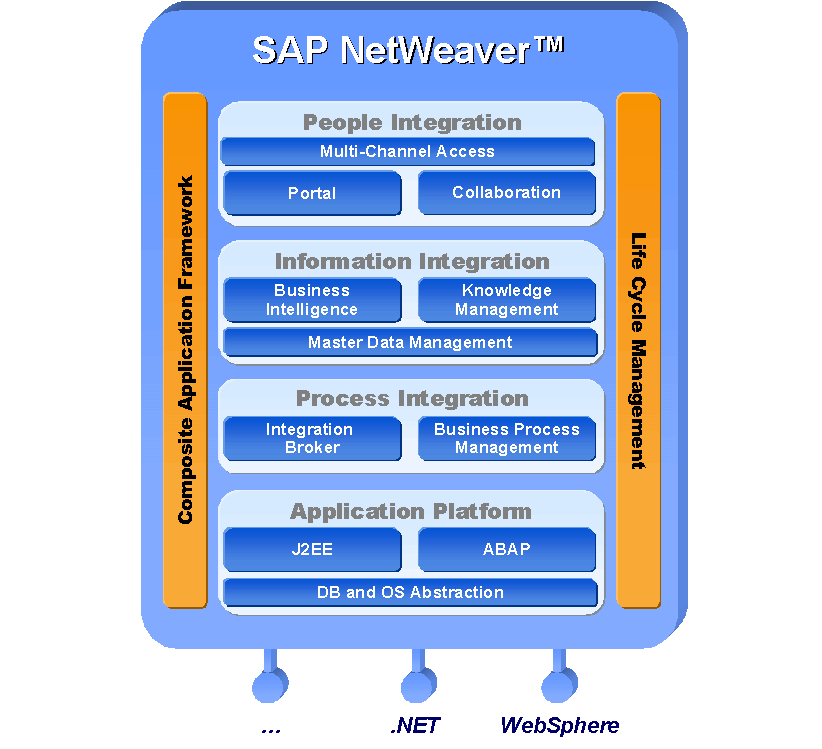
\includegraphics[width=1\linewidth]{grafiken/NetWeaver.png}
	\vspace{-20pt}
	\caption{Aufbau der \gls{sap} \gls{nw} Plattform (Quelle: \cite{NWGrundlagen})}
	\vspace{-10pt}
	\label{abb:SAPNWGrundlagen}
	\end{center}
\end{figure}

Über alle Bereiche gibt es das Life Cycle Management und das Composite Application Framework. Life Cycle Management umfasst Design, Entwicklung, Test, fortlaufender Betrieb der Applikationen und dessen Administrations- \gls{bzw} Change-Management. Daher bietet \gls{nw} Life Cycle Manamgent für alle der Vier Bereiche an.
Das Composite Application Framework ermöglicht es, Applikationen aus verschiedenen Bereichen für \gls{nw} zu entwickeln.

%%%%%%%%%%%%%%%%%%%%%%%
%% KAPITEL Datenbank %%
%%%%%%%%%%%%%%%%%%%%%%%
%% STEFFEN
%%%%%%%%%%%%%%%%%%%%%%%
\section{Datenbanken}
Ein \gls{sap}-System stellt generell nur die Anwendungssoftware zur Verfügung. Die notwendigen Daten werden in einer (externen) \gls{db} bereitgestellt. Daher ist die Auswahl der \gls{db} genauso wichtig, wie die Auswahl der Hardware-Plattform und des Betriebssystems.
Die \gls{sap} Datenbank ist eine Ansammlung an verbundenen Tabellen, die als \gls{rdbms} bekannt ist. Manche Produkte, wie zum Beispiel \gls{erp}, bestehen aus mehr als 40.000 Tabellen \cite{SAPin24hrs}.

\subsection{SAP HANA}
\label{sec:db-hana}

\subsubsection{Einführung}
\label{sec:db-hana-intro}
% historische, hana studio, rowstore (anderer Aufbau als bei herkömml. dbs)
\gls{sap} \gls{hana} kombiniert die Funktionen einer \gls{db}, der Datenverarbeitung und die Funktionen einer Anwendungsplattform auf Ebene des Hardware Arbeitsspeichers. \gls{hana} bietet \gls{ua} Bibliotheken für Vorhersage, Planung, Textanalyse oder Geschäftsanalysen an.\\

\begin{figure}[H]
	\begin{center}
	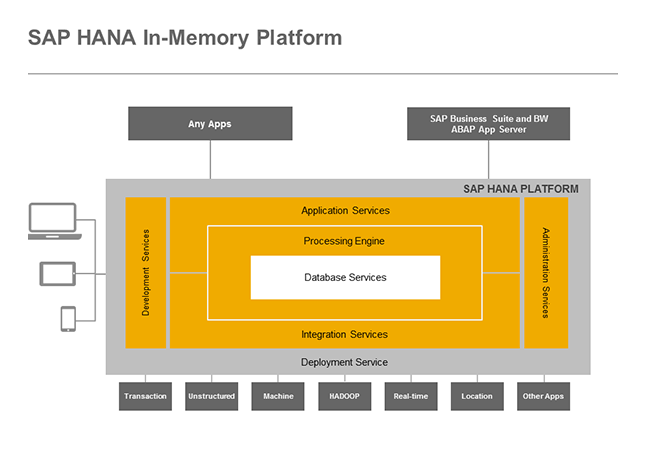
\includegraphics[width=1\linewidth]{grafiken/hana-features-overview.png}
	\vspace{-20pt}
	\caption{Aufbau der \gls{sap} \gls{hana} Plattform \cite{SAPHanaAbout}}
	\vspace{-10pt}
	\label{abb:SAPHanaAbout}
	\end{center}
\end{figure}

\gls{hana} verwendet in seiner \gls{db} einen sogenannten spaltenbasierten Datenspeicher, welcher im Arbeitsspeicher abgespeichert wird. Dieser Datenspeicher ist durch verschiedene Sicherheitsfeatures vor Datenverlust bei Stromausfall oder ähnlichem gesichert.
Dadurch, dass Anwendungen direkt auf der \gls{hana} Instanz ausgeführt werden können, vereinfacht es die Entwicklung von Applikationen im Umfeld von großen Datenmengen. In Abbildung \ref{abb:SAPHanaAbout} ist die Struktur von \gls{hana} abgebildet. Hier wird gezeigt, dass \gls{hana} nicht nur eine \gls{db} ist, sondern weitaus mehr.

\subsubsection{Hands On}
\label{sec:db-hana-ho}
% welche wichtigen Befehle gibt es
Für dieses Kapitel wurde eine \gls{hana} Instanz von Grund auf konfiguriert und für den Einsatz vorbereitet. 
Als Grundlage für unser Testsystem dient ein mit VMWare virtualisierter Server mit folgenden Spezifikationen
\begin{itemize}
	\item \gls{cpu} \ldots Intel(R) Xeon(R) CPU E7- 4870  @ 2.40GHz mit 10vCores
	\item \gls{ram} \ldots 127 Gigabyte
	\item \gls{hdd} \ldots 180 Gigabyte
	\item \gls{os} \ldots Suse Enterprise Linux 11.2	
\end{itemize}

Aufgrund von Komplexitäts- und Zeitgründen gehe ich an dieser Stelle nicht weiter auf die Installation der \gls{hana} Instanz ein, lediglich ist zu erwähnen, dass man gewisse Instanz Attribute zum späteren Login benötigt. Dies sind \gls{ua} \emph{Instance}, \emph{Sid} und natürlich Logindaten für den \emph{System} Benutzer.\\
Zum benutzen der \gls{hana} Instanz benötigt man das Programm "`\gls{sap} \gls{hana} Studio"'. Dieses steht unter folgendem Link\footnote{\url{http://scn.sap.com/community/developer-center/hana}} zum Download zur Verfügung.

Nachdem das System im \gls{hana} Studio (mithilfe der Instanz Attribute) hinzugefügt wurde, können alle Funktionen von \gls{hana} verwenden werden.

Zunächst befüllen wir eine Datenbank mit mehreren Tabellen, die mit Hilfe eines \gls{sql} Scripts mit Zufallsdaten gefüllt werden (siehe \ref{anhang:hanasql}). In unserem Beispiel werden 10 Millionen Datensätze eingefügt. Um zu prüfen, wie viele Datensätze eine Tabelle enthält gehen wir wie in \ref{hana:countselect} dargestellt vor.

\lstset{language=SQL, caption={Beispieldaten zählen}, label={hana:countselect}}								
\begin{lstlisting}
	SELECT count(*) FROM "SYSTEM"."TABLENAME"
\end{lstlisting}

Aufgrund der Komplexität des Scripts dauerte das Einfügen auf unserer \gls{hana} Testmaschine mehr als 40 Stunden. Dies kann je nach Hardware deutlich variieren.\\

\lstset{language=SQL, caption={Beispieldaten selektieren}, label={hana:select}}								
\begin{lstlisting}
	SELECT * FROM "SYSTEM"."TABLENAME"
\end{lstlisting}

Um alle 10 Millionen Datensätze zu selektieren (Listing \ref{hana:select}), benötigt die \gls{hana} \gls{db} lediglich weniger als 285 Millisekunden. Dies zeigt, dass auch weitaus mehr Datensätze selektiert und damit Anwendungen exponentiell im Vergleich zu herkömmlichen \gls{db} verschnellert werden können. Wie sich \gls{hana} im Vergleich mit anderen herkömmlichen \gls{db} verhält, wird in Kapitel \ref{sec:db-hana-vgl} behandelt.

\begin{center}
	\begin{verbatim}
		Statement 'SELECT * FROM "SYSTEM"."SALES_F"' 
		successfully executed in 284 ms 214 µs  
		(server processing time: 275 ms 793 µs)
	\end{verbatim}
\end{center}

\subsubsection{Vergleich}
\label{sec:db-hana-vgl}
% zeitvergleich oracle / hana db select
Zum praktischen Vergleich mit der öffentlich verfügbaren und häufig im Web-Bereich verwendeten MySQL \gls{db}, wurden Testdatensätze von MySQL\footnote{\url{https://dev.mysql.com/doc/employee/en/employees-installation.html}} in eine MySQL \gls{db} eingefügt. Eine der Tabellen enthält \emph{2.844.047} Datensätze. Somit ist ein vergleichbares Ergebnis erzielbar. Leider ist die hießig verwendete Hardware weitaus schlechter als die verwendete Hardware für \gls{hana}. Nichtsdestotrotz ist ein Vergleich an dieser Stelle durchaus repräsentabel. Mithilfe von der Programmiersprache PHP selektieren (Listing \ref{anhang:mysql-select}) wir die Datensätze und zeigen uns die Dauer der Selektion an. 
MySQL benötigt also für die \emph{2.844.047} Datensätze ca. \emph{3.32} Sekunden. Somit ist die \gls{hana} \gls{db} mehr als 41 mal schneller als die MySQL \gls{db}.

\subsection{Sonstige}
\label{sec:db-sonstige}
% welche datenbanken kann man sonst benutzen
% oracle,...
\gls{sap} unterstützt unter anderem Microsoft \gls{sql}-Server, \gls{sql} Azure, \gls{ibm} DB2 und die Oracle-Datenbank. Weiterhin unterstützt \gls{sap} natürlich seine eigenen Datenbanken MaxDB, Sybase und die zuvor behandelte \gls{hana}.

\chapter{SAP Workflow Builder}  \label{chap:builder}
%%%%%%%%%%%%%%%%%%%%
%% KAPITEL Intro %%
%%%%%%%%%%%%%%%%%%%
\section{Einführung}
% MARCO
% was ist es, wer benutzt es, wofür braucht man es
% erreichbar durch Transaktion SWDD, im SAP System eingebaut usw
%%%%%%%%%%%%%%%%%%%%%%%%%%%%%%%%%%%%%%%%%%%%%%%%%%%%%%%%%%%%%%%%%
% http://www.connexin.net/de/sap-transaktionen-uebersicht.html
% -> Hier auch die Workflow transaktionen mit LOG etc erwähnen!
% http://help.sap.com/saphelp_nw04s/helpdata/EN/c5/e4b79d453d11d189430000e829fbbd/content.htm
% -> Bild zum Beispiel für die Übersicht des Builders zu erklären
% http://www.sdn.sap.com/irj/scn/go/portal/prtroot/docs/library/uuid/3c2b9c90-0201-0010-ab86-a574c7881607?QuickLink=index&overridelayout=true&5003637211723
% -> schöne Definitionen und Übersicht des Builders
% http://www.edv-buchversand.de/sap/chapter.php?cnt=getchapter&id=gp-9285.pdf
% -> auch sehr gut für Übersicht!!
% http://www.abap-tutorials.com/wp-content/uploads/pdfs/workflow_tutorial.pdf
% -> geil für die Einführung mit Warum brauchen wir überhaupt Workflows etc..
\subsection{Warum ein SAP Workflow Builder?}
\label{sec:warum-wf-builder}
Durch eine sehr breite Produktpalette und lange Erfahrung ist in einem \gls{sap} System standardmäßig eine sehr große Menge an Arbeitsabläufen vorhanden und direkt einsetzbar. Aufgrund der Verschiedenheit individueller Firmen und Branchen ist es allerdings unmöglich, alle möglichen Workflows zu integrieren und zur Verfügung zu stellen. Daher stellt die \gls{sap} ihren Kunden eine Möglichkeit zur Verfügung, mit der sie, nach einer gewissen Einarbeitungszeit, beliebige Workflows selbst abbilden können. Dadurch können gekaufte Produkte mit einer maximalen Genauigkeit in die vorhandenen Betriebsabläufe integriert und auch schon vorhandene Fremdsysteme angesprochen werden \cite{SAPHelpWf}.

\subsubsection{Vorteile des SAP Workflow Builders}
\label{sec:vorteile-sap-wf-builder}
Durch die direkte Einbindung in das \gls{sap} System hat der Workflow Builder einige Möglich\-keiten und Funktionen, die mit einem externen Programm nicht umsetzbar wären. So ist es möglich, auf interne Ereignisse zu warten und auf diese zu reagieren. Des weiteren können auch globale Ereignisse ausgelöst werden und es kann problemlos mit anderen \glspl{transaktion} des Systems zusammengearbeitet werden. 

Da viele Firmen zur Verwaltung der Produktion, des Personals und anderen Dingen größtenteils \gls{sap} Systeme im Einsatz haben, ist es somit möglich, ein Maximum an Automatisierung zu erreichen.

\subsection{Programmoberfläche}
\label{sec:win-overwiev}
Die Programmoberfläche des Workflow Builders (Abbildung \ref{abb:workflow-overview}) ist in verschiedene Bereiche unterteilt. Die wichtigsten sind die im Folgenden beschriebenen.

\begin{figure}[h]
	\begin{center}
	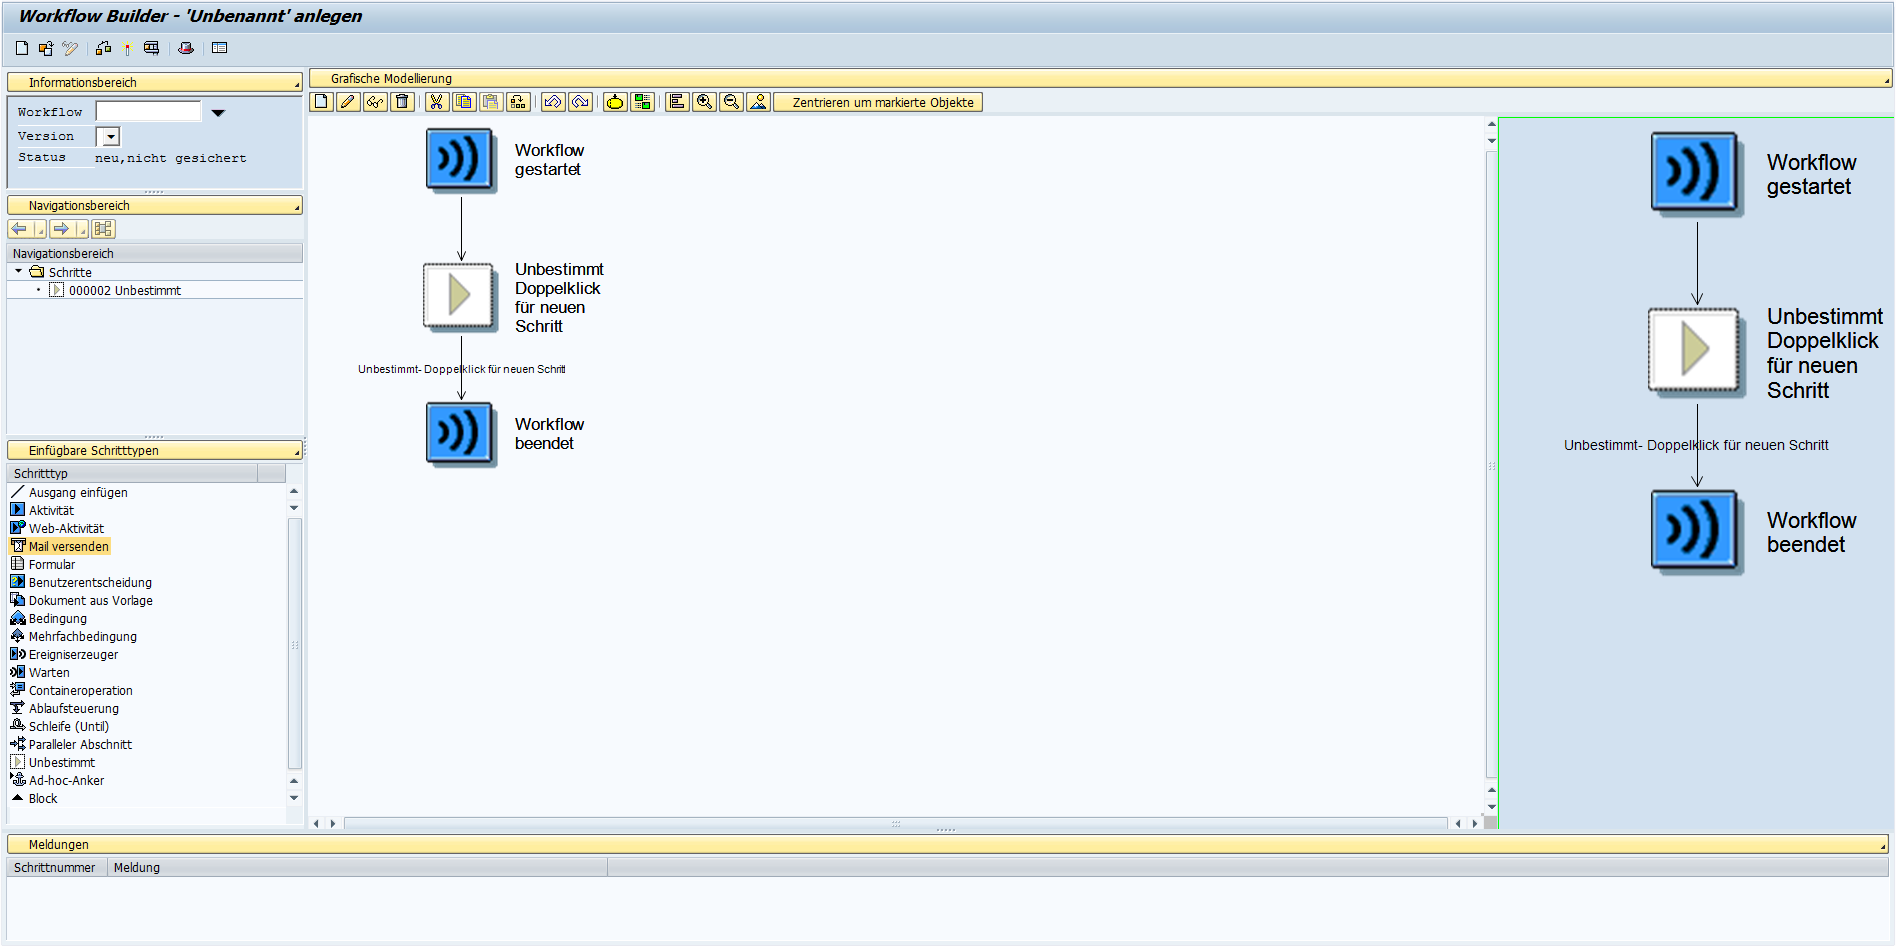
\includegraphics[width=1.0\textwidth]{grafiken/wf-builder_overview.png}
	\caption{Programmübersicht: Der SAP Workflow Builder}
	\vspace{-10pt}
	\label{abb:workflow-overview}
	\end{center}
\end{figure}

\subsubsection{Workflow}
\label{sec:win-overview-wf}
Dieser Bereich ist der wichtigste und größte. Hier wird der Bereich des modellierten Arbeitsablaufs, der gerade bearbeitet wird, groß dargestellt und es können neue Schritte eingefügt werden, vorhandene Schritte editiert oder gelöscht werden. Ein Doppelklick auf einen Schritt bringt den Benutzer zur gespeicherten Definition des Elements, welche dort gepflegt werden kann.

\subsubsection{Übersicht}
\label{sec:win-overview-uebersicht}
Die grafische Übersicht bietet dem Bearbeiter stets einen Überblick des gesamten Workflows, wofür dieser bei großen Modellierungen stark verkleinert dargestellt werden muss. Zusätzlich signalisiert ein grüner rechteckiger Rahmen stets, welcher Teil des Gesamtbildes aktuell im großen Workflow Fenster bearbeitet wird. Durch Verschieben des Rahmens ist es möglich, direkt zu einem gewünschten Teil zu springen.

\subsubsection{Schritttypen}
\label{sec:win-overview-schrittypen}
Der untere linke Bereich des Programms hat standardmäßig den Titel "`Einfügbare Schrittypen"' und enthält eine Liste aller Schrittypen, die verwendet werden können. Von hier können diese mit der Maus per \gls{dragdrop} in den Prozess eingefügt werden. Beim Einfügen des Schrittes wird durch ein kleines Plus am Mauszeiger signalisiert, dass der entsprechende Schritt an dieser Stelle eingefügt werden kann.

\subsubsection{Informationsbereich}
\label{sec:win-overview-information}
Der Informationsbereich zeigt an, welcher Workflow aktuell geladen ist, dessen Status und Versionsnummer. Durch einen Klick auf die Auswahlliste neben "`Version"' kann eine andere Version des gespeicherten Prozesses geladen werden. Um einen neuen Prozess zu laden, kann entweder, wenn diese bekannt ist, die entsprechende Identifikationsnummer in das Textfeld neben "`Workflow"' eingegeben werden oder die Suchhilfe mittels des kleinen Pfeils daneben geöffnet werden. Letzteres öffnet das in Abbildung \ref{abb:workflow-search} gezeigte Fenster, in welchem die auf dem System vorhandenen Workflows nach Kategorien aufgegliedert angezeigt werden.

\begin{figure}[h]
	\begin{center}
	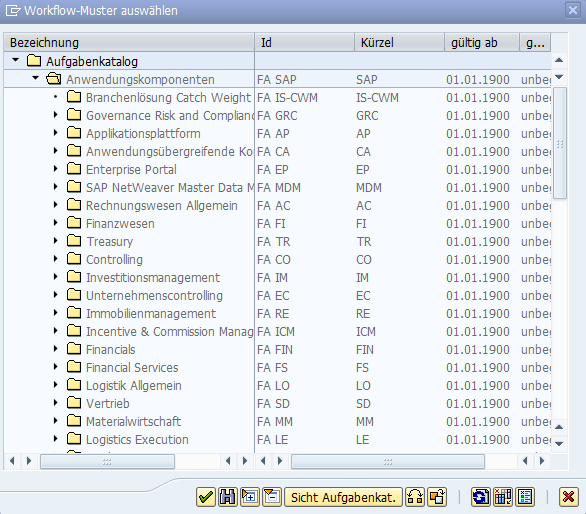
\includegraphics[width=300px]{grafiken/wf-builder_search.png}
	\caption{Suchhilfe des Workflow Builders}
	\vspace{-10pt}
	\label{abb:workflow-search}
	\end{center}
\end{figure}

\subsubsection{Navigationsbereich}
\label{sec:win-overview-information}
Der Navigationsbereich beinhaltet eine Liste aller im Prozess vorhandenen Schritte. Von hier aus ist es möglich, direkt zu der Definition eines gewünschten Schrittes zu springen. 

\subsubsection{Meldungen}
\label{sec:win-overview-meldungen}
In diesem Bereich werden Nachrichten zur Information des Benutzers angezeigt. Dies können allgemeine Benachrichtigungen, Ergebnisse der Syntaxprüfung oder Suchergebnisse sein.

\subsubsection{Alternative Inhalte}
\label{sec:win-overview-alternative}
Zusätzlich zu den standardmäßig beim Programmstart und in Abbildung \ref{abb:workflow-overview} angezeigten Informationen kann die Ansicht \nameref{sec:win-overview-schrittypen} zu einer alternativen Ansicht geändert werden. Dies erfolgt, indem der Benutzer auf die Überschrift "`Einfügbare Schritttypen"' des Bereichs klickt. Aus dem nun geöffneten Menü (Abbildung \ref{abb:workflow-alternatives}) ist einer der Einträge auszuwählen. Die folgenden Ansichten stehen zur Verfügung:

\begin{figure}[h]
	\begin{center}
	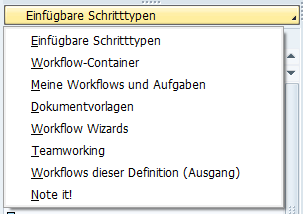
\includegraphics[width=220px]{grafiken/wf-builder_alternative-inhalte.png}
	\caption{Alternative Anzeigemöglichkeiten des Workflow Builders}
	\vspace{-10pt}
	\label{abb:workflow-alternatives}
	\end{center}
\end{figure}

\begin{enumerate}
	\item Der \textbf{Workflow Container} beinhaltet alle Elemente, wie Variablen und Benutzereingaben, welche während der Ausführung des Workflows benötigt werden. Neben den automatisch generierten Container Elementen können auch vom Benutzer definierte Elemente angelegt werden.
	\item Die Ansicht \textbf{Meine Workflows und Aufgaben} bietet einen Schnellzugriff auf alle Workflows, die in letzter Zeit bearbeitet wurden. Des weiteren kann eine eigene Liste an Aufgaben und Workflows angelegt werden.
	\item \textbf{Dokumentvorlagen} sind Dokumente externer Programme (Excel-Tabellen, Word-Dateien oder beliebige andere), welche im Schritt "`Dokument aus Vorlage"' eingebunden werden können. 
	\item \textbf{Workflow Wizards} bieten dem Benutzer die Möglichkeit, häufig genutzte Prozessteile mit Hilfe eines von \gls{sap} bereitgestellten \gls{wizard}s einzufügen.
	\item In der Ansicht \textbf{Teamworking} kann nach Schritten gesucht werden, welche von einer bestimmten Person als letztes bearbeitet wurden.
	\item Der Punkt \textbf{Workflows dieser Definition (Ausgang)} zeigt alle zur Zeit auf dem System ausgeführten Instanzen dieser Workflow Version.
	\item Der letzte Punkt, \textbf{Note it!} bietet dem Benutzer die Möglichkeit, sich Notizen zu seiner aktuellen Arbeit zu erstellen.
\end{enumerate}

\subsection{Funktionen des Builders}
\label{sec:builder-funktionen}
% MARCO
% welche Funktionalitäten hat der Builder...
Im Folgenden sollen nun zuerst die wichtigsten Funktionen des \gls{sap} Workflow Builders erklärt werden. Danach folgt im Kapitel \nameref{sec:builder-elemente} eine breiter gefächerte tabellarische Übersicht. Dort sind auch die Symbole der Schrittypen mit aufgeführt. 

Beim ersten Start des Programms wird dem Benutzer statt einer leeren Arbeitsfläche der minimale Aufbau eines Workflows im \gls{sap}-System angezeigt (Abbildung \ref{abb:workflow-easy}). Dieser besteht aus dem Startereignis "`Workflow gestartet"' und dem Endereignis "`Workflow beendet"'. Dazwischen können beliebige Schritte an Stelle des unbekannten Schrittes (gekennzeichnet durch einen Pfeil auf weißem Hintergrund) eingefügt werden.

\begin{figure}[h]
	\begin{center}
	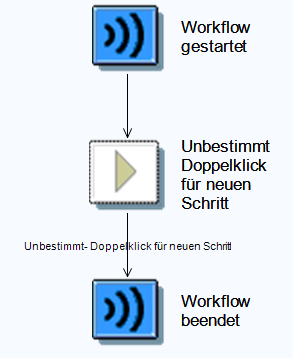
\includegraphics[width=150px]{grafiken/wf-builder_new-wf.png}
	\caption{Initialer Workflow des Builders}
	\vspace{-10pt}
	\label{abb:workflow-easy}
	\end{center}
\end{figure}

\subsubsection{Aktivität}
Der wichtigste Schritttyp ist die Aktivität, welche verschiedene Aufgaben erfüllen kann. Der Benutzer kann entweder einen \gls{abap} \gls{objekttyp} und eine zugehörige Methode oder eine im System vorhandene und schon definierte Aufgabe auswählen. Die entsprechende Aktivität wird dann vom System automatisch gestartet, wenn die Stelle im laufenden Workflow erreicht wird \cite{SAPHelpWf}.

\subsubsection{Web-Aktivität}
Mit Hilfe dieses Schrittes wird aus dem internen Workflow heraus ein \gls{xml}-Dokument an eine URL gesendet. Der Empfänger kann beispielsweise ein anderes System sein, welches daraufhin einen eigenen Workflow startet. Alle \gls{sap}-Systeme stellen einen Service zur Verfügung, welcher in diesem Fall automatisch einen weiteren Workflow starten kann \cite{SAPHelpWf}.

\subsubsection{Mail versenden}
Dieser Schritt versendet eine Nachricht innerhalb des \gls{sap}-Systems. Der Empfänger (es sind mehrere Empfänger möglich) kann diese im internen Postfach abrufen. Der Text der Mail wird bei der Definition des Schrittes festgelegt, wobei Variablen verwendet werden können, welche zur Laufzeit mit den entsprechenden Werten gefüllt werden \cite{SAPHelpWf}.

\subsubsection{Formular}
Ein Formular kann innerhalb des Workflows zur Anzeige von Daten oder deren Bearbeitung durch den Endnutzer verwendet werden. Nachdem bei der Definition des Schrittes die zu bearbeitenden Daten angegeben wurden, erzeugt das Workflow-System automatisch das zugehörige Formular, welches noch bearbeitet werden kann \cite{SAPHelpWf}. 

\subsubsection{Benutzerentscheidung}
Eine Benutzerentscheidung kann mit einem Text versehen werden, welcher dem Endnutzer erklärt, welche Entscheidung er treffen muss. Der Workflow kann so konfiguriert werden, dass er, je nachdem welche der vorgegebenen Antwortmöglichkeiten ausgewählt wurde, einen anderen Pfad wählt \cite{SAPHelpWf}.

\subsubsection{Bedingungen}
Die Schritte Bedingung und Mehrfachbedingung bestimmen, ähnlich der Benutzerentscheidung, den weiteren Ablauf des Workflows. Der Unterschied besteht darin, dass das System die Entscheidung eigenständig nach vorgegebenen Bedingungen fällt und der Benutzer keinen Einfluss darauf hat \cite{SAPHelpWf}.

\subsubsection{Schleifen}
Die \emph{WHILE}- und \emph{UNTIL}-Schleifen können eingesetzt werden, wenn ein bestimmter Teil des Workflows ausgeführt werden soll, während eine bestimmte Bedingung wahr ist oder so lange, bis sie eintritt. Schleifen können sämtliche Schrittypen (auch weitere Schleifen) enthalten und sorgen dafür, dass ein Workflow übersichtlich bleibt \cite{SAPHelpWf}.

\subsection{Verschiedene Ansichten}

Zur besseren Übersichtlichkeit und Darstellung, welche Funktionen die einzelnen Schritte eines Workflows haben, arbeitet der \gls{sap} Workflow Builder mit eigenen Symbolen und einer daraus resultierenden eigenen Ansicht. Dies ist leicht erkennbar in Abbildung \ref{abb:workflow-bsp1-complete} des Anhangs, welche den beispielhaften Workflow zeigt, der später in Kapitel \ref{sec:builder-1-bsp} erarbeitet wird. Um eine möglichst große Kundengruppe anzusprechen und zufrieden zu stellen, bietet der Workflow Builder noch weitere Ansichten, welche den allgemeinen Normen entsprechen. Um auf eine dieser Ansichten umzustellen, wählt der Benutzer aus dem Menü \textit{Zusätze} den Punkt \textit{Optionen}, woraufhin er im sich nun öffnenden Dialogfeld (Abbildung \ref{abb:workflow-change-view}) aus dem Menü der Zeile \textit{Sicht} die gewünschte Ansicht auswählen kann. Zu erwähnen ist die Ansicht \textit{Klassische ereignisgesteuerte Prozessketten (ClassicEPCs)} (Abbildung \ref{abb:workflow-view-classicepc}), welche aus der Geschäftsprozesse-Vorlesung bekannt sind und eine Mischform aus der \gls{sap}-eigenen Ansicht und den \textit{ClassicEPCs}, den sogenannten \textit{EPCs} (Abbildung \ref{abb:workflow-view-epc}). Diese Mischform ist sinnvoll, wenn eine bessere Orientierung mit Hilfe der \gls{sap} Symbole gewünscht ist und nicht auf die Darstellung durch klassische \gls{epk} verzichtet werden soll. Die kompakte Ansicht ist nur eine geringfügig platzsparendere Version der Standardansicht.

\begin{figure}[h]
	\begin{center}
	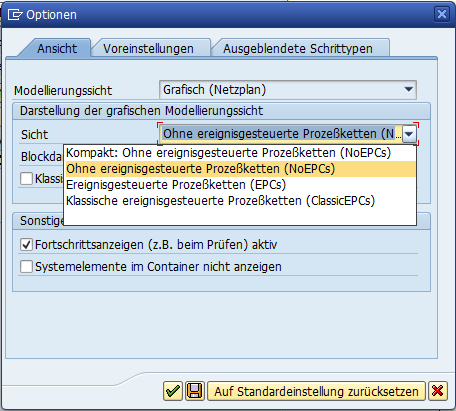
\includegraphics[width=300px]{grafiken/wf-builder_options-change-view.png}
	\caption{Ändern der Ansicht des Workflow Builders}
	\vspace{-10pt}
	\label{abb:workflow-change-view}
	\end{center}
\end{figure}

\subsection{Schritttypen}
\label{sec:builder-elemente}
% MARCO, STEFFEN
% tabelle mit elementen..
% was ist wofür gedacht
	\begin{longtable}{|c|p{2.5cm}|p{10.5cm}|}
		\hline
		\textbf{Symbol} & \textbf{Schritttyp} & \textbf{Beschreibung}\\
		\hline
		\includegraphicstotab[width=0.8cm]{grafiken/aktivitaet.png}
		& 
		Aktivität & Ausführen einer ABAP-Methode oder einer vordefinierten Aufgabe \\ 
		\hline \includegraphicstotab[width=0.8cm]{grafiken/web-aktivitaet.png} 
		& 
		Web-Aktivität & \gls{xml}-Dokument an eine URL senden, z.B. um Workflows in Fremdsystemen zu starten\\ 
		\hline 
		\includegraphicstotab[width=0.8cm]{grafiken/mail-versenden.png} 
		& 
		Mail-Versendung & Nachricht an Endnutzer versenden\\ 
		\hline 
		\includegraphicstotab[width=0.8cm]{grafiken/formular.png}
		& 
		Formular\-schritt & Anzeige von Daten und Möglichkeit zum Bearbeiten dieser durch Endnutzer\\ 
		\hline 
		\includegraphicstotab[width=0.8cm]{grafiken/benutzerentscheidung.png}
		& 
		Benutzer\-entscheidung & Beantworten einer Frage bzw. Treffen einer Entscheidung durch den Benutzer zur Beeinflussung des Workflows\\ 
		\hline 
		\includegraphicstotab[width=0.8cm]{grafiken/dokument-aus-vorlage.png}
		& 
		Dokument aus Vorlage & Anzeigen oder Bearbeiten von Dokumenten, die mit externen Anwendungen erstellt wurden mit Hilfe eines auf dem Rechner installierten Programms\\ 
		\hline 
		\includegraphicstotab[width=0.8cm]{grafiken/bedingung.png}
		& 
		Bedingung & Bedingte, selbstständige Entscheidung für einen Pfad aus zwei Möglichkeiten durch das System\\ 
		\hline 
		\includegraphicstotab[width=0.8cm]{grafiken/mehrfachbedingung.png}
		& 
		Mehrfach\-bedingung & Bedingte, selbstständige Entscheidung für einen Pfad aus mehreren Möglichkeiten durch das System\\ 
		\hline 
		\includegraphicstotab[width=0.8cm]{grafiken/ereigniserzeuger.png}
		& 
		Ereignis\-erzeuger & Auslösen eines Ereignisses, auf welches ein Warteschritt wartet\\ 
		\hline 
		\includegraphicstotab[width=0.8cm]{grafiken/warten.png}
		& 
		Warteschritt & Warten, bis ein durch einen Ereigniserzeuger generiertes Ereignis eintritt\\ 
		\hline 
		\includegraphicstotab[width=0.8cm]{grafiken/containeroperationen.png}
		& 
		Container\-operationen & Verändern von Elementen des Workflow-Containers (Umgebung des aktiven Workflows mit Variablen und Benutzerentscheidungen)\\ 
		\hline 
		\includegraphicstotab[width=0.8cm]{grafiken/ablaufsteuerung.png}
		& 
		Ablauf\-steuerung & Eingriff in den Ablauf des aktuellen Workflows - Abbruch oder Beenden einzelner Schritte oder des gesamten Workflows\\ 
		\hline 
		\includegraphicstotab[width=0.8cm]{grafiken/schleife.png}
		& 
		Schleifen & Mehrfache Ausführung eines Blocks von Schritten unter einer bestimmten Bedingung\\ 
		\hline 
		\includegraphicstotab[width=0.8cm]{grafiken/paralleler-abschnitt.png}
		& 
		Paralleler Abschnitt & Aufsplitten des Workflows in zwei parallel laufende Pfade\\ 
		\hline 
		\includegraphicstotab[width=0.8cm]{grafiken/ad-hoc-anker.png}
		& 
		Ad-hoc-Anker & Möglichkeit, einen anderen Workflow des Systems zu hinterlegen, der vom berechtigten Benutzer ausgeführt werden kann\\ 
		\hline 
		\includegraphicstotab[width=0.8cm]{grafiken/block.png}
		& 
		Block & Zusammenfassen mehrerer Schritte zu einem Block mit eigenen Variablen\\ 
		\hline 
		\includegraphicstotab[width=0.8cm]{grafiken/lokaler-workflow.png}
		& 
		Lokaler Workflow & Einfügen eines Sub-Workflows, welcher vollen Zugriff auf die Daten des aktuellen Workflows hat\\ 
		\hline 
		% Beschriftung festlegen:
		\caption{Symbolerklärung des \gls{sap} Workflow Builders}
		% ein Label definieren, mit dessen Hilfe man (an beliebiger Stelle im 	Dokument) Bezug nehmen kann:
		\label{tab:builderelemente}
\end{longtable}

%%%%%%%%%%%%%%%%%%%%%
%% KAPITEL HandsOn %%
%%%%%%%%%%%%%%%%%%%%%
%% MARCO
%%%%%%%%%%%%%%%%%%%%%
\section{Hands On}
In diesem Kapitel soll die Arbeit mit dem \gls{sap} Workflow Builder näher beleuchtet werden, indem zwei beispielhafte Prozesse zuerst in der Theorie erklärt und danach im System gebaut werden. Um eine Steigerung zu erreichen, wird die Kreation des ersten, sehr einfachen Workflows Schritt für Schritt beschrieben, wohingegen beim zweiten, etwas komplexeren Workflow darauf verzichtet wird, jede Eingabe zu erklären. Stattdessen wird dessen grobere Funktionsweise erläutert. 

\subsection{Erstes Beispiel: Kontrolle des Materials}
\label{sec:builder-1-bsp}
% kleiner sinnloser workflow (schleife,...) => aus dem Video Tutorial

\subsubsection{Vorstellung des Workflows}
\label{sec:builder-1-bsp-vorstellung}
Zum Einstieg soll ein Workflow angelegt werden, welcher einen sehr geringen Funktionsumfang hat. Dieser besteht aus folgenden Punkten:

\begin{itemize}
	\item Der Workflow soll automatisiert starten, sobald der Benutzer ein neues Material im System anlegt.
	\item Als erstes wird der Benutzer gefragt, ob er das soeben angelegte Material noch einmal kontrollieren will.
	\item Im Falle einer Entscheidung für "`ja"' wird das erzeugte Material angezeigt.
	\item Entscheidet sich der Benutzer gegen eine Anzeige des Materials, soll er darüber per E-Mail informiert werden.
\end{itemize}

Dieser Ablauf ergibt, gerade unter Betrachtung der Information per E-Mail darüber, dass das angelegte Material nicht angezeigt werden soll, nicht zwangsläufig einen Sinn, um ihn in einer existierenden Firma anzuwenden, soll aber stattdessen die Arbeit mit Startereignissen, Benutzerentscheidungen und weiteren Aktivitäten erklären.

\subsubsection{Umsetzung des Workflows}
\label{sec:builder-1-bsp-umsetzung}
Um den beschriebenen Workflow im Builder umzusetzen ist es sinnvoll, zuerst den Ablauf ohne Startereignis oder Datenübergabe zu erstellen. Zur Vereinfachung wird daher vorerst davon ausgegangen, dass bereits bekannt ist, um welches Material es geht, so wird nur von "`dem Material"' gesprochen. 

Als erstes soll der Benutzer gefragt werden, ob er das soeben erstellte Material anzeigen möchte. Dazu wird der Schritt \textit{Benutzerentscheidung} per \gls{dragdrop} auf das leere Feld zwischen dem schon vorhandenen Start- und Endereignis gezogen. Daraufhin öffnet sich das Formular zur Konfiguration der Abfrage. Als Text soll hier beispielsweise eingegeben werden "`Wollen Sie das Material anzeigen?"'. Als mögliche Entscheidungsalternativen sollen in der unteren Hälfte des Formulars "`Ja, ich will"' und "`Nein, danke"' mit den zugehörigen Ausgangsbezeichnungen "`ja"' und "`nein"' angegeben werden. Der Bearbeiter der Abfrage soll der Workflow Initiator sein. Hierzu wird im Menü unter "`Bearbeiter"' der entsprechende Ausdruck eingefügt. (Abbildung \ref{abb:workflow-bsp1-benentsch_form}) Dies ist die Person, welche den Workflow gestartet hat. Der Bearbeiter ist die Person, welche später die Abfrage per E-Mail erhält.

\begin{figure}[h]
	\begin{center}
	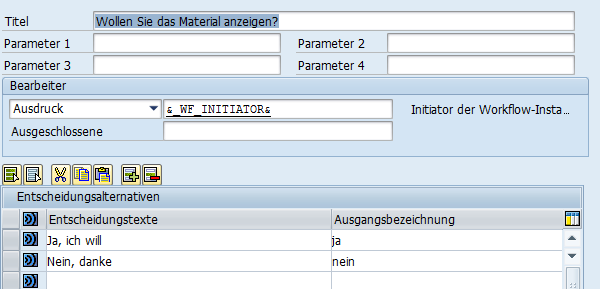
\includegraphics[width=400px]{grafiken/wf-builder_bsp1_formular-benutzerentscheidung.png}
	\caption{Ausgefülltes Formular zur Benutzerentscheidung}
	\vspace{-10pt}
	\label{abb:workflow-bsp1-benentsch_form}
	\end{center}
\end{figure}

Nachdem die Benutzerentscheidung eingefügt wurde, teilt das System den bisher linearen Pfad in zwei Teile, die mit den angegebenen Kurztexten der Antwortmöglichkeiten versehen sind. Da der Benutzer im Falle einer Entscheidung für "`nein"' eine E-Mail erhalten soll, wird nun der Schritt \textit{Mail versenden} auf den entsprechenden Pfad gezogen. Im nun folgenden Eingabefeld muss nur der Text und der Betreff der Mail ausgefüllt werden. Wird als Empfängerart "`Organisationsobjekt"' und wieder der Workflow Initiator ausgewählt, so wird die Nachricht innerhalb des \gls{sap} Systems versendet. (Abbildung \ref{abb:workflow-bsp1-mail_form})

\begin{figure}[h]
	\begin{center}
	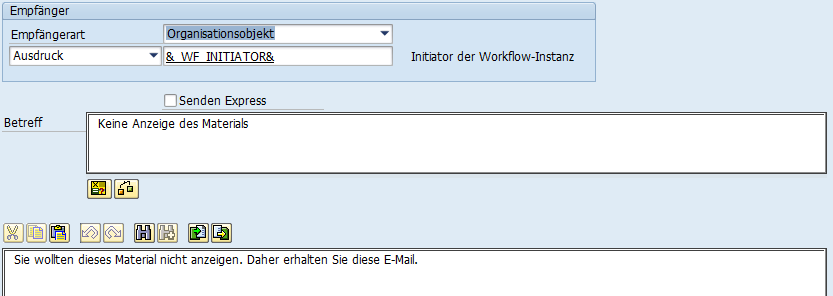
\includegraphics[width=400px]{grafiken/wf-builder_bsp1_formular-mail.png}
	\caption{Das ausgefüllte Formular zur internen Mail}
	\vspace{-10pt}
	\label{abb:workflow-bsp1-mail_form}
	\end{center}
\end{figure}

Der letzte noch fehlende Punkt im Prozess ist die eigentliche Anzeige des Materials. Hierzu wird der Schritt \textit{Aktivität} auf den noch verbleibenden, leeren Pfad nach der Benutzerentscheidung gezogen. Die Konfiguration dieses Schrittes ist etwas aufwändiger, da für jede Aktivität, sofern noch nicht vorhanden, eine Aufgabe angelegt werden muss. Dies kann erledigt werden, indem das Menü neben dem Schriftzug "`Aufgabe"' geöffnet und der Eintrag "`Aufgabe anlegen"' ausgewählt wird. Im nun angezeigten Formular (Abbildung \ref{abb:workflow-bsp1-aufgaben_form}) muss der neuen Aufgabe nun ein Kürzel und eine Bezeichnung zugewiesen werden. Da es im \gls{sap} System den vorgefertigten \gls{bor} Objekttypen "`Standard Material"' gibt, ist es für den Benutzer nicht von Nöten, eine eigene \gls{abap} Klasse hierfür zu erstellen. Als Objektkategorie kann "`\gls{bor}-Objekttyp"' ausgewählt und als Objekttyp \\\texttt{BUS1001006} eingegeben werden. Ist der Objekttyp nicht bekannt, kann hier die im \gls{sap} System global verfügbare Eingabehilfe verwendet werden. Mit dieser kann danach auch aus den verfügbaren Methoden des Objekttypen gewählt werden. Im konkreten Fall wird die Methode \texttt{DISPLAY} verwendet.

\begin{figure}[h]
	\begin{center}
	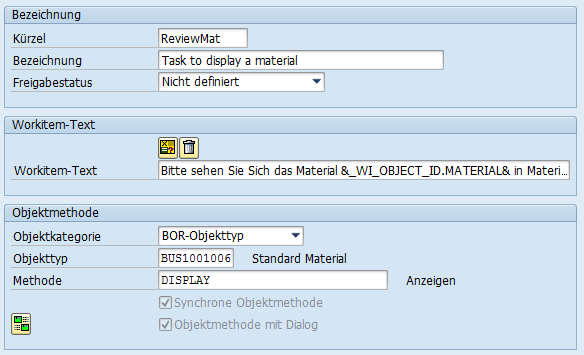
\includegraphics[width=400px]{grafiken/wf-builder_bsp1_formular-aufgabe.png}
	\caption{Ausgefülltes Formular zur neuen Aufgabe}
	\vspace{-10pt}
	\label{abb:workflow-bsp1-aufgaben_form}
	\end{center}
\end{figure}

Letztlich sollte im Feld \textit{Workitem-Text} noch ein Text angegeben werden, der dem Endnutzer beschreibt, was zu erledigen ist. Mit dem entsprechenden Button 
\includegraphics[height=1em]{grafiken/wf-builder_bsp1_formular-aufgabe_btn_eingabehilfe-ausdruck.png} links neben dem Papierkorb über dem Eingabefeld können hierzu Variablen aus einer zusätzlichen Eingabehilfe (Abbildung \ref{abb:workflow-bsp1-aufgaben_form-inputhelp}) eingefügt werden.

Nach dem Speichern der Aufgabe aber vor dem Schließen des Aufgabeneditors sollte noch eine letzte Option getroffen werden. Diese definiert die Aufgabe als generelle Aufgabe, was bedeutet, sie kann von jedem Benutzer des Systems ausgeführt werden. Die Pflege des Bearbeiters erfolgt über das Menü in der Titelleiste des \gls{sap} Programms. Hierzu wird das Menü \textit{Zusatzdaten} - \textit{Bearbeiterzuordnung} - \textit{Pflegen} aufgerufen und nach einem Klick auf \textit{Eigenschaften...} die Auswahl "`Generelle Aufgabe"' getroffen. Über den normalen zurück-Button des Systems kann nun zum Bearbeiten der Aktivität zurück gesprungen werden. Dort ist, wie bei den vorigen Elementen auch, als Bearbeiter der Workflow Initiator einzustellen. 

Sind sämtliche Einstellungen getroffen und es wird wieder das Hauptfenster inklusive des Workflows angezeigt, so muss als letzte Einstellung noch dafür gesorgt werden, dass das Objekt "`Material"' beim Starten des Workflows importiert wird. Dies ist nötig, da das Objekt nicht im Laufe des Prozesses generiert wird, sondern dieser gestartet wird, nachdem ein Material angelegt wurde. Um diese Änderung durchzuführen, muss der Benutzer, wie in Kapitel \ref{sec:win-overview-alternative} beschrieben, zur Ansicht der Workflow-Container wechseln, den oben beschriebenen Container "`BUS1001006"' mit einem Doppelklick öffnen und dort im Reiter \textit{Eigenschaften} das Kästchen vor "`Import"' anhaken (Abbildung \ref{abb:workflow-bsp1-containeredit-import} des Anhangs).

Nach diesem Schritt, nachdem er gespeichert 
\includegraphics[height=1em]{grafiken/btn_sap_save.png}, geprüft 
\includegraphics[height=1em]{grafiken/btn_sap_check.png} und aktiviert 
\includegraphics[height=1em]{grafiken/btn_sap_activate.png} wurde, kann de Workflow in der Testumgebung des Builders zum ersten Mal ausgeführt 
\includegraphics[height=1em]{grafiken/btn_sap_excecute.png} werden. 

Nun sind von den in Kapitel \ref{sec:builder-1-bsp-vorstellung} genannten Punkten alle bis auf den ersten umgesetzt. Um den Prozess automatisiert zu starten, sobald ein neues Material angelegt wird, benötigt der Workflow ein sogenanntes \textit{Startereignis}. Diese können in einem Formular gepflegt werden, welches über das Kontextmenü \textit{Springen} - \textit{Grunddaten} unter dem Reiter \textit{Startereignisse} erreichbar ist. Um ein neues Startereignis anzulegen sind die folgenden Einstellungen zu treffen:

\begin{itemize}
	\item In der Spalte \textbf{Kategorie} muss festgelegt werden, dass es sich um ein \gls{bor}-Objekt handelt. 
	\item Naheliegenderweise muss in der Spalte \textbf{Objekttyp} der bereits bekannte Typ \texttt{BUS1001006} angegeben werden.
	\item Das auszuwählende \textbf{Ereignis des Objekts} ist \texttt{CREATED}.
	\item Über einen Klick auf den linken der drei gelben Buttons muss das Ereignis \textbf{aktiviert} werden.
	\item Letztlich muss der \textbf{Datenfluss} über den mittleren Button 
\includegraphics[height=1em]{grafiken/wf-builder_bsp1_btn-datenfluss.png} und einem Druck auf den grünen Haken 
\includegraphics[height=1em]{grafiken/btn_sap_apply.png} aktiviert werden, sodass beim Erstellen eines Materials die Materialnummer an den Workflow Container übergeben wird.
\end{itemize}

Der erstelle Workflow ist nun nach einer weiteren Aktivierung (siehe oben) der getroffen Definition fertiggestellt und kann verwendet werden. Er sollte vom System, wie in Abbildung \ref{abb:workflow-bsp1-complete} gezeigt, dargestellt werden und startet sich nun automatisch, sobald über die \gls{transaktion} \texttt{MM01} ein Material angelegt wird. Den Workflow erhält der entsprechende Benutzer standardmäßig in seinen \gls{businessworkplace} ausgeliefert, sodass er diesen dort starten kann.

\subsection{Zweites Beispiel: Erstellung und Genehmigung einer Abwesenheitsnachricht}
\label{sec:builder-2-bsp}
% demo workflow aus den vorlagen nehmen (abwesenheitsbestätigung)

\subsubsection{Vorstellung des Workflows}
\label{sec:builder-2-bsp-vorstellung}
% wofür ist der workflow gut, was soll er tun (aus anwendersicht)
Als zweites, etwas komplexeres Beispiel soll der Prozess der Abwesenheitsnachricht dienen. In diesem Prozess erstellt der Angestellte einer Firma direkt nach dem Start des Workflows eine Abwesenheitsmitteilung mit Hilfe eines vorgegebenen Formulars. Daraufhin erhält der Vorgesetzte des Angestellten eine Mitteilung in sein internes Postfach, welche den Hinweis enthält, dass er die Mitteilung bearbeiten soll. Hiernach soll es zwei Möglichkeiten geben. Erfolgt eine Genehmigung, soll der Antragsteller benachrichtigt werden. Im Falle einer Ablehnung muss der Workflow Initiator die Wahl haben, die Mitteilung zu überarbeiten oder zu löschen. Im Falle einer Überarbeitung muss der Prozess ab der Genehmigung erneut beginnen.

\subsubsection{Umsetzung des Workflows}
\label{sec:builder-2-bsp-umsetzung}
% technische sicht, "`klickbares"' howto
Nachdem in Kapitel \ref{sec:builder-1-bsp-umsetzung} die Umsetzung sehr genau beschrieben wurde und die Konfiguration einzelner Aktivitäten und Benutzerentscheidungen bekannt ist, soll dieser Prozess nun vom logischen Ablauf her betrachtet werden und die entsprechende Umsetzung im \gls{sap} System aufgezeigt werden.

Die Idee hinter der Logik dieses Workflows ist ein sogenanntes Flag, welches eine Art Variable darstellt, welche durch zwei verschiedene Zustände aufzeigt, ob die Bearbeitung der Abwesenheitsmitteilung abgeschlossen ist oder die Bearbeitungsschleife erneut durchlaufen werden muss. Dieses Flag wird im schon bekannten \textit{Workflow Container} angelegt und ist eine \gls{abap}-Dictionary-Referenz des Feldes \texttt{RETURNCODE} der Struktur \texttt{SWD\_LINES}. Die Konfiguration des Containerelements kann in Abbildung \ref{abb:workflow-bsp2-container-flag} eingesehen werden. Ein zusätzliches Container-Element ist das eigentliche Formular zur Anzeige und Bearbeitung einer Abwesenheitsmitteilung. Dieses Formular ist ein im System standardmäßig vorhandener \gls{bor} Objekttyp mit dem Namen \texttt{FORMABSENC} und kann somit einfach angelegt werden (Abbildung \ref{abb:workflow-bsp2-container-form}). 

Nachdem die beiden benötigten Elemente des Containers angelegt wurden und somit das nötige Umfeld steht, kann nun der eigentliche Workflow erstellt werden. Zum einfachen Nachbau des Prozesses ist die Konfiguration der einzelnen Aufgaben jeweils im Anhang abgebildet. 

Wie bereits in Kapitel \ref{sec:builder-2-bsp-vorstellung} erwähnt, soll nach dem Start des Workflows eine Abwesenheitsmitteilung angelegt werden. Dies wird durch eine entsprechend konfigurierte Aktivität erreicht, wobei die benötigte Aufgabe bereits im System unter dem Kürzel \texttt{exformabscre} vorhanden ist und der Bearbeiter der Workflow Initiator ist. Als Schrittbezeichnung wählen wir \textit{AM anlegen}. (Abbildung \ref{abb:workflow-bsp2-act_am-anlegen})

Der noch folgende Rest des Prozesses soll, wie in Kapitel \ref{sec:builder-2-bsp-vorstellung} beschrieben, komplett wiederholt werden, sofern der Benutzer sich später für die erneute Überarbeitung der Mitteilung entscheidet. Daher wird nun eine Schleife eingefügt, sodass sämtliche noch folgenden Schritte direkt in diese eingebaut werden können. Dies verhindert späteres Umbauen des Workflows beim nachträglichen Einfügen der Schleife. Wurde die benötigte \textit{Schleife (Until)} am entsprechenden Platz im Prozess eingefügt, so öffnet sich das Konfigurationsfenster derselben. Die Bedingung kann, da das benötigte Flag bereits erstellt wurde, mit Hilfe einfach mit der entsprechenden Eingabehilfe (Abbildung \ref{abb:workflow-bsp2-act_loop_inputhelp}) eingefügt werden. Die komplette Konfiguration der Schleife kann in Abbildung \ref{abb:workflow-bsp2-act_loop} eingesehen werden.

Anhand der nächsten Aktivität zur Genehmigung oder Ablehnung der Abwesenheit wird klar, dass eine Aktivität, je nach Konfiguration der entsprechenden Aufgabe dahinter, mehr als einen Ausgang haben kann. Nachdem die Aufgabe eingetragen wurde, bleibt noch die Konfiguration des Bearbeiters. Da die Genehmigung dem Vorgesetzten obliegt, kann hier nicht, wie gewohnt, der Workflow Initiator eingetragen werden. Da die Person, welche die Aufgabe bearbeiten soll beim Erstellen des Prozesses noch nicht bekannt ist, sondern vom Workflow Initiator abhängt, wird aus dem Menü unter Bearbeiter der Wert \textit{Regel} ausgewählt und die im System unter dem Kürzel \texttt{saf\_manager} vorhandene Regel zum finden eines Vorgesetzten in das Textfeld dahinter eingetragen. (Abbildung \ref{abb:workflow-bsp2-act_am-genehmigen_klein}) Die Konfiguration der kompletten Aufgabe ist in Abbildung \ref{abb:workflow-bsp2-act_am-genehmigen} einsehbar.

\begin{figure}[h]
	\begin{center}
	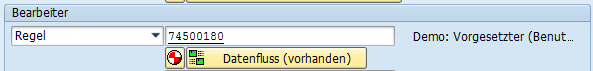
\includegraphics[width=1.0\textwidth]{grafiken/wf-builder_bsp2_act_am-genehmigen_klein.png}
	\caption{Verwenden der Regel zum Auswählen des Vorgesetzten}
	\vspace{-10pt}
	\label{abb:workflow-bsp2-act_am-genehmigen_klein}
	\end{center}
\end{figure}

Dem Pfad \textbf{genehmigt} nach der letzten Aufgabe soll ein Schritt eingefügt werden, der das oben erwähnte Flag so setzt, dass die Ausführung des Prozesses von der eingebundenen Schleife nicht wiederholt wird. Dieser Schritt kann einfach über den Schritttypen \textit{Containeroperation} erledigt werden, indem das \textit{Ergebniselement} mit Hilfe der entsprechenden Zuweisung auf den Ausdruck \texttt{000} gesetzt wird (Abbildung \ref{abb:workflow-bsp2-act_flag-0000}). Anschließend soll das System automatisiert mit Hilfe der entsprechenden Aufgabe (Abbildung \ref{abb:workflow-bsp2-act_message-genehmigt}) eine Benachrichtigung über die Genehmigung versenden.

\begin{figure}[h]
	\begin{center}
	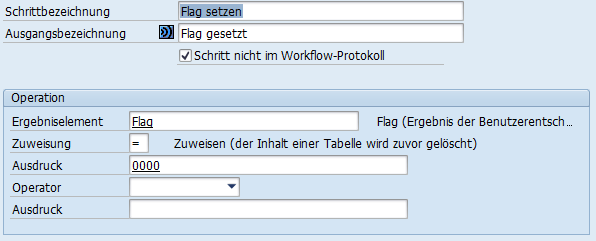
\includegraphics[width=0.75\textwidth]{grafiken/wf-builder_bsp2_act_flag_0000.png}
	\caption{Setzen des Flags auf den Wert 0}
	\vspace{-10pt}
	\label{abb:workflow-bsp2-act_flag-0000}
	\end{center}
\end{figure}

Nachdem der erste Pfad nun vollständig mit den nötigen Schritten befüllt wurde, soll der Workflow Initiator nun im Pfad \textbf{abgelehnt} danach gefragt werden, wie er weiter vorgehen möchte. Die gegebenen Möglichkeiten sind das Löschen oder das Überarbeiten der Abwesenheitsmitteilung. Da diese Entscheidung zwar den weiteren Verlauf des Prozesses beeinflusst, allerdings nicht, wie die Genehmigung, in einer Datenbank festgehalten werden muss, kann dieser Schritt durch eine simple \textit{Benutzerentscheidung} gelöst werden. Innerhalb dieser Entscheidung kann zur besseren Übersicht im Titel der Abfrage die Nummer der Abwesenheitsmitteilung angegeben werden. Dies erfolgt durch ein kaufmännisches Und als Platzhalter und dem Eintragen des entsprechenden Parameters in die Parameterliste darunter. Die entsprechende Konfiguration, die ähnlich schon in Kapitel \ref{sec:builder-1-bsp-umsetzung} erklärt wurde, kann in Abbildung \ref{abb:workflow-bsp2-act_was-tun} eingesehen werden. Auch nach dieser Entscheidung teilt das System den Pfad wieder in zwei weitere Pfade auf, welche wie folgt konfiguriert werden.

Der Pfad \textbf{löschen} wird mit einer Aktivität und der entsprechenden Aufgabe \texttt{AF\_delete} zum Löschen einer Mitteilung (Abbildung \ref{abb:workflow-bsp2-act_am-loeschen}) und der Containeroperation zum Setzen des Flags, wie in Abbildung \ref{abb:workflow-bsp2-act_flag-0000} gefüllt. Wird der Pfad \textbf{überarbeiten} eingeschlagen, so ist ein Setzen des Flags nicht nötig, da der Workflow ein weiteres Mal durchlaufen werden muss. Der Benutzer soll allerdings davor mit Hilfe einer Aktivität und der Aufgabe \texttt{AF\_update} die Möglichkeit erhalten, seine Mitteilung zu bearbeiten. (Abbildung \ref{abb:workflow-bsp2-act_am-editieren})

%%%%%%%%%%%%%%%%%%%%%%%%%%
%% KAPITEL Fremdsysteme %%
%%%%%%%%%%%%%%%%%%%%%%%%%%
%% JONAS 
%%%%%%%%%%%%%%%%%%%%%%%%%%
\section{Schnittstellen}

\subsection{SAP Fremdsysteme}
\label{sec:export-sap}

\gls{sap} Systeme liefern Workflows, die auf das Ziel der Applikation ausgelegt sind. \gls{erp}, \gls{crm} und \gls{srm} sind Beispiele für Systeme, die eingebaute, vordefinierte Workflows bereitstellen. 

Die Workflows sind anpassbar, um den Bedürfnissen der Firma gerecht zu werden. Es können mit dem Workflow Builder ganz eigene Geschäftsprozesse entwickelt werden, die natürlich über Modulgrenzen hinweg Zugriff auf Daten besitzen. So können Daten aus einem \gls{crm}-System in einem \gls{erp} zur Analyse, Auswertung und Bearbeitung von Daten hinzugezogen werden.

\subsection{XML}
\label{sec:export-xml}
% was ist dieses Format
% in welche Programme kann man es importieren?

\gls{xml} ist die Abkürzung für E\textbf{x}tensible \textbf{M}arkup \textbf{L}anguage und bezeichnet eine Auszeichnungssprache. Mit dieser können hierarchisch strukturierte Daten in Textform dargestellt werden. \gls{xml} besteht aus Elementen, deren Name, bis auf ein paar Ausnahmen, frei gewählt werden darf. Elemente haben einen Anfangs- ($\langle$elementName$\rangle$) und einen Endtag ($\langle$/elementName$\rangle$). Zwischen den Tags können weiter Elemente, Text und Knoten stehen. Diese sind dem Element dann untergeordnet.

Das World Wide Web Consortium, kurz \gls{w3c}, hat \gls{xml} als eine Metasprache definiert, auf deren Basis anwendungsspezifische Auszeichnungssprachen entwickelt werden können. Diese werden beschrieben durch ein Schema, welches festlegt, welche Elemente verwendet werden dürfen und welches Verhalten diese aufweisen \cite{XML}. So ist \gls{zb} auch XHTML definiert.

\subsection{BPMN und BPML}
\label{sec:export-bpmn-bpml}
% was ist dieses Format
% in welche Programme kann man es importieren?

\textbf{B}usiness \textbf{P}rocess \textbf{M}odel and \textbf{N}otation (\gls{bpmn}) ist eine grafische Spezifikationssprache, welche Symbole bereitstellt mit deren Hilfe Geschäftsprozesse und Arbeitsabläufe dargestellt werden können \cite{BPMN}. \gls{bpmn} wurde 2005 von der \gls{omg}, auch zuständig für \gls{zb} \gls{uml}, übernommen und gewann ab dann an Bedeutung in der Informatik. Außerdem wurde sie 2013 zum internationalen Standard (ISO/IEC 19510:2013) erhoben \cite{OMG}.

Da sich \gls{bpmn} rein auf die Darstellung von Workflows bezieht wurden mehrere, von \gls{xml} abgeleitete, Auszeichnungssprachen entwickelt, um Business Process Models auch als, für einen Computer verständliche, Daten aufschreiben zu können. Dazu zählen \gls{zb} \gls{bpel}, \gls{xpdl} oder \gls{bpml} \cite{BPMN}.

Die \textbf{B}usiness \textbf{P}rocess \textbf{M}odeling \textbf{L}anguage (\gls{bpml}) wird von \gls{sap} im Workflowbuilder (\ref{chap:builder}) verwendet um Geschäftsprozesse zu exportieren. Da \gls{bpml} auch unter dem Dach der \gls{omg} steht wird sie auch in anderen Workflow Management Systemen, wie \gls{zb} jBPM, Camunda BMP oder ARIS, verwendet. Dadurch lassen sich \gls{sap}-interne Geschäftsprozesse auch extern einbetten \cite{BPML}.

\chapter{SAP Business By Design}  \label{chap:byd}
%%%%%%%%%%%%%%%%%%%
%% KAPITEL Intro %%
%%%%%%%%%%%%%%%%%%%
%% JONAS         %%
%%%%%%%%%%%%%%%%%%%
\section{Einführung}

\gls{sap} \gls{byd} ist die \gls{erp} \gls{ondemand} Cloudlösung für \gls{sme} (\ref{sec:byd}).

Für Installation, Wartung und Aktualisierung der Lösung sorgt das integrierte Betriebsmodell. Alle Betriebskosten, die durch ein Vor-Ort System entstehen sind also im Preis einbegriffen. Damit kann sich der Kunde vollständig auf sein Kerngeschäft konzentrieren.

\gls{sap} \gls{byd} wird über eine sichere Internetverbindung und einen Webbrowser als dynamische Website aufgerufen. Somit können User von überall auf ihren Arbeitsplatz zugreifen und müssen weder vor Ort im Büro sein noch sich anderweitig ins Firmennetz einwählen.

\subsubsection{Vorteile von \gls{byd}}

\begin{itemize}
\item \gls{byd} vereinigt alle Vorteile einer modernen Unternehmensanwendung bei minimalen Anforderungen an die IT
\item \gls{byd} greift auf bewährte Geschäftsvorfälle zurück, die umgehend einsatzbereit sind
\item Der Kunde hat automatisch Zugriff auf die aktuellste Softwareversion des Produkts
\item \gls{byd} schont die Investition für eine eigene IT-Infrastruktur durch ein skalierbares Mietmodell
\item Die Lösung kann leicht an wechselnde Geschäftsanforderungen angepasst werden.
\end{itemize}
\cite{itelligence}

%%%%%%%%%%%%%%%%%%%%%%%%%%%%%%%%
%% KAPITEL Benutzeroberfläche %%
%%%%%%%%%%%%%%%%%%%%%%%%%%%%%%%%
%% JONAS                      %%
%%%%%%%%%%%%%%%%%%%%%%%%%%%%%%%%
\section{Benutzeroberfläche}

\begin{figure}[H]
	\begin{center}
	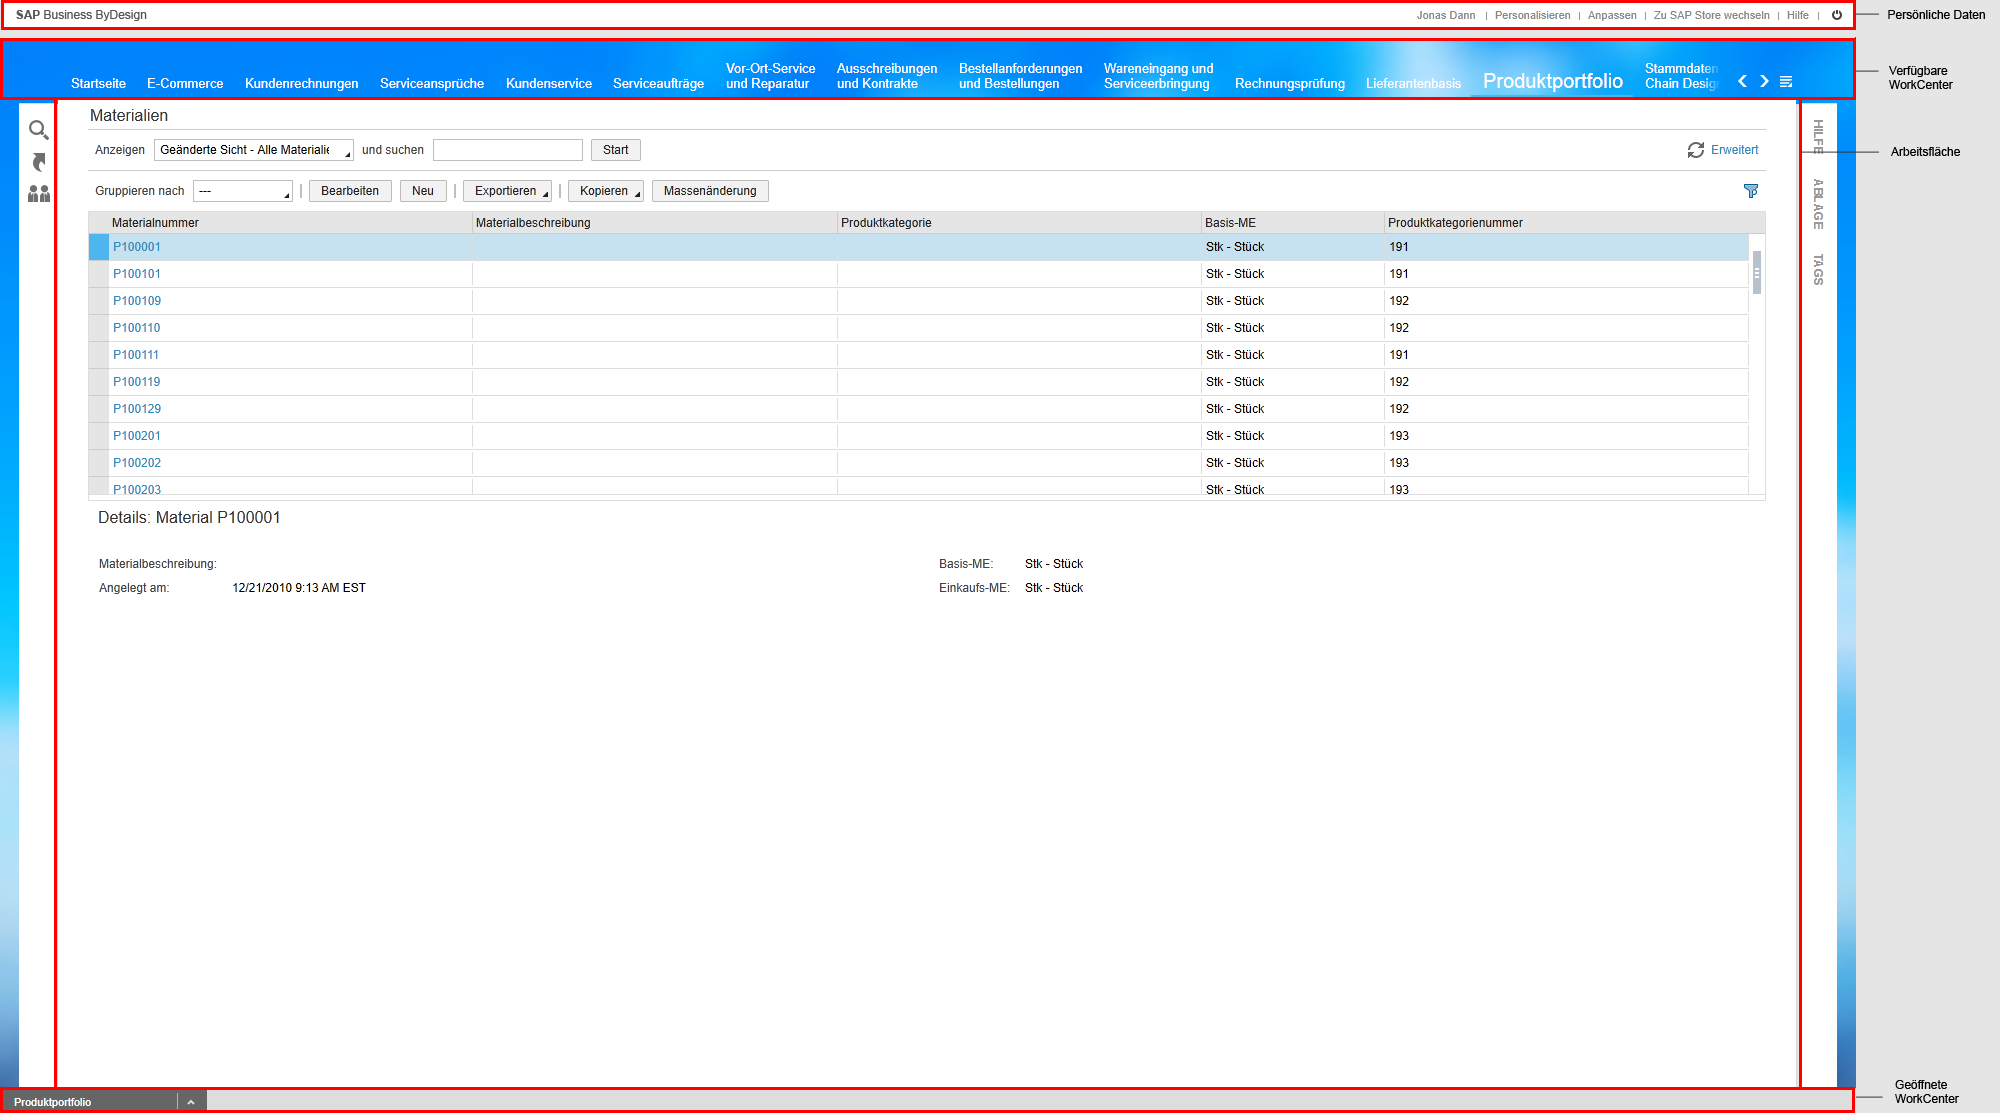
\includegraphics[width=1.0\textwidth]{grafiken/ByDesign-Ubersicht.png}
	\caption{ByDesign Übersicht}
	\vspace{-10pt}
	\label{abb:byd-overview}
	\end{center}
\end{figure}

\subsubsection{Persönliche Daten}

Hier kann der User seine Daten, wie \gls{zb} Telefonnummer oder E-Mail, einstellen. Außerdem kann er seine Benutzeroberfläche in \gls{byd} personalisieren. Weiterhin besteht die Möglichkeit in den \gls{sap}-Store zu wechseln und eine Hilfsseite aufzurufen.

\subsubsection{Verfügbare WorkCenter}

\gls{byd} ist in verschiedene WorkCenter unterteilt, die jeweils einen Teilgeschäftsprozess abbilden. So kann man \gls{zb} seine Mitarbeiter oder Waren verwalten.

In dieser Sektion der Anzeige kann der User die verschiedenen für ihn verfügbaren WorkCenter auswählen. Diese werden dann unten im "`Geöffnete WorkCenter"' Bereich angezeigt und in der Arbeitsfläche geöffnet.

\subsubsection{Arbeitsfläche}

Hier werden die eigentlichen Inhalte des Webinterfaces angezeigt. Wenn der Beispielworkflow durchgespielt wird, werden auch nur noch diese Ausschnitte des Bildschirms gezeigt.

\subsubsection{Geöffnete WorkCenter}

Im Bereich "`Geöffnete WorkCenter"' sieht der User alle WorkCenter, die er im Moment geöffnet hat. Die Anzeige funktioniert wie Tabs in einem Webbrowser und der Nutzer kann damit zwischen verschiedenen Ansichten und Aufgaben wechseln.

%%%%%%%%%%%%%%%%%%%%%%%%%%%%%%
%% KAPITEL Beispielworkflow %%
%%%%%%%%%%%%%%%%%%%%%%%%%%%%%%
%% JONAS                    %%
%%%%%%%%%%%%%%%%%%%%%%%%%%%%%%
\section{Beispielworkflow}

\subsection{Vorstellung des Workflows}
\label{sec:byd-bsp-vorstellung}
% Schulungsworkflow beschreiben (anwendersicht)

\subsubsection{Szenario}

Der Verkaufsbereichsleiter einer Firma hat auf einer Technologiemesse ein innovatives Produkt entdeckt. Er würde gerne einen neuartigen Solarboiler in das Produktportfolio der Firma aufnehmen. Die Nachfrage nach Innovation und neuen Produkten ist sehr groß.

\subsubsection{Aufgaben des Mitarbeiters}

\begin{enumerate}
 \item Er sucht einen Anbieter für das gewünschte Produkt.
 \item Danach ermittelt er über Preisvergleiche die günstigsten Anbieter, die gleichzeitig auch eine hohe Verfügbarkeit gewährleisten sollen.
 \item Er fügt das Produkt in \gls{byd} ein und ordnet ihm eine Produktkategorie zu.
 \item Nach der Zuordnung müssen alle wichtigen Daten in das System eingepflegt werden.
 \item Nun fügt er die erforderlichen Angaben über jeden Anbieter in \gls{byd} ein.
 \item Nachdem er die Anbieter angelegt hat, fordert er Angebote an.
 \item Nach Erhalt werden diese in \gls{byd} eingepflegt.
 \item Es können dann die Angebote verglichen werden und gegebenenfalls wird der Zuschlag erteilt und ein Vertrag geschlossen.
 \end{enumerate}

\subsection{Umsetzung des Workflows}
\label{sec:byd-bsp-umsetzung}
% technische sicht, "`klickbares"' howto

\subsubsection{Anbietersuche}

Im ersten Schritt werden Anbieter des gewünschten Produktes \gls{zb} auf der Website Alibaba\footnote{\url{alibaba.com}} gesucht. Auf dieser Website können kleine Unternehmer ihre Produkte zum Verkauf anbieten. Im Moment sind über 2 Millionen Anbieter registriert.

Für dieses Beispiel wird der SunSurf SC-IP01\footnote{\url{http://www.alibaba.com/product-detail/SunSurf-SC-IP01-solar-boiler-system_627442099.html?s=p}} Solar Boiler verwendet. Dieser kostet zwischen 400 und 500 USD(\$) und muss mindestens zu 15 Stück bestellt werden. Der Anbieter kann maximal 5000 Stück im Monat liefern.

\subsubsection{Produkt im System anlegen}

Im WorkCenter "`Produktportfolio"' können nun die Daten des SunSurf SC-IP01 unter einem neuen Material abgespeichert werden. Dazu klickt der User auf "`Produkte nach Materialien"' und dann auf "`Neu"'. In dem folgenden Formular werden dann die Daten des Solar Boilers angegeben (Abbildung \ref{abb:byd-newmaterial}).

Nachdem auf "`Sichern und schließen"' geklickt wurde, wurde das Produkt erfolgreich angelegt.

\subsubsection{Anbieter anlegen}

Im WorkCenter "`Lieferantenbasis"' unter "`Lieferanten"' legt der User einen neuen Anbieter an. Dazu klicken er wieder auf "`Neu"' und gibt dann im Formular die Daten des Anbieters ein (Abbildung \ref{abb:byd-newsupplier}).

Nachdem er auf "`Sichern und schließen"' geklickt hat wurden die Eingaben erfolgreich angelegt.

\subsubsection{Angebotsanforderung versenden}

Es ist alles vorbereitet um eine Ausschreibung zu erstellen. Dies geschieht im WorkCenter "`Ausschreibungen und Kontrakte"'. Dort wählt der User "`Ausschreibungen und Angebote"' aus. Er klickt auf "`Neu"' und füllen die allgemeinen Daten der Ausschreibung (Abbildung \ref{abb:byd-rfq-1}). 

Danach können die Produkte hinzugefügt werden, die mit der Ausschreibung behandelt werden sollen (Abbildung \ref{abb:byd-rfq-2}).

Als letztes fügt der Nutzer die Bieter ein, die automatisch über ihre Teilnahme an der Ausschreibung benachrichtigt werden (Abbildung \ref{abb:byd-rfq-3}).

\subsubsection{Angebot entgegennehmen}

Wenn die Bieter Angebote vorlegen, können diese über eine Eingabemaske in \gls{byd} eingegeben werden (Abbildung \ref{abb:byd-rfq-4}). Dabei werden allgemeine Daten und Preise des Bieters eingepflegt werden (Abbildung \ref{abb:byd-rfq-5}).

\subsubsection{Vertrag/Kontrakt schließen}

Sämtliche Angebote können in einer Gesamtansicht angezeigt und verglichen werden (Abbildung \ref{abb:byd-rfq-6}). Dem besten Angebot wird der Zuschlag erteilt. 
Die Entscheidung erscheint auf dem Arbeitsplatz des Vorgesetzten als offene Aufgabe. Dieser kann den Kontrakt dann schließen oder ablehnen (Abbildung \ref{abb:byd-contract}).

%%%%%%%%%%%%%%%%%%%%%
%% KAPITEL Grenzen %%
%%%%%%%%%%%%%%%%%%%%%
%% JONAS           %%
%%%%%%%%%%%%%%%%%%%%%
\section{Grenzen von ByD}

\subsubsection{Vordefinierte Geschäftsprozesse}

Die Idee eine vorkonfigurierte On-Demand Unternehmensmanagement Applikation weist Nachteile gegenüber den anderen \gls{sme}-Lösungen im Bereich Customizing auf. So kann \gls{byd} nicht beliebig granular konfiguriert werden, da die Geschäftsabläufe von \gls{sap} standardisiert vorgegeben werden.

\subsubsection{Module}

Da \gls{byd} in Form von Modulen zusammengestellt ist, erhält der Kunde unausweichlich auch Funktionalität, die er nicht nutzt und bezahlt damit für unnötige Anwendungsbestandteile. In diesem Aspekt sind Business One \ref{sec:business-one} oder \gls{sap} All-in-One \ref{sec:allinone} die bessere Wahl.

\subsubsection{Erweiterbarkeit}

Im Gegensatz zu den beiden anderen \gls{sme}-Systemen kann \gls{byd} nicht beliebig erweitert werden. So können nicht einfach spezifische Prozesse neu entwickelt und in das vorhandene System eingebunden werden, da \gls{byd} keine Möglichkeit bietet eigene Workflows anzulegen und auch \gls{sap} keine weit über die Standardsoftware hinausgehenden Add-Ons anbietet.



\chapter{Gesamtfazit}  \label{chap:fazit}
% irgendwie einmal ByD und Workflow Builder zusammenfassen (jeweils Jonas & Marco)
% ein kleinen Abschnitt dass ByD f�r Firmen besser ist, die mit fest definierten Prozessen einverstanden sind
% und keine eigenen brauchen, als auch f�r kleine Firmen. F�r gro�e, die viel Customizing brauchen
% ist Workflow Builder weitaus besser, da viel mehr Individualisierbar und Komplexer
% jeder Wunsch kann damit erf�llt werden. Perfekte Implementierung in vorhandene SAP Landschaft

\appendix
\chapter{Anhang}  \label{chap:anhang}
%%%%%%%%%%%%%%%%%%%%
%% KAPITEL ANHANG %%
%%%%%%%%%%%%%%%%%%%%
\section{HANA Beispieldaten}

\lstset{language=SQL, caption={Beispieldaten anlegen \cite{SAPSCN}}, label={anhang:hanasql}}								
\begin{lstlisting}
CREATE COLUMN TABLE "SALES_F" ("SALES_ORDER_NBR" BIGINT CS_FIXED NOT NULL ,
       "CALENDAR_DAY" DAYDATE CS_DAYDATE,
       "BUSINESS_UNIT_ID" BIGINT CS_FIXED,
       "MATERIAL_ID" BIGINT CS_FIXED,
       "SUPPLIER_ID" BIGINT CS_FIXED,
       "UNIT_PRICE" DOUBLE CS_DOUBLE,
       "QUANTITY_SOLD" DOUBLE CS_DOUBLE,
       PRIMARY KEY ("SALES_ORDER_NBR"));

CREATE COLUMN TABLE "BUSINESS_UNIT_D" ("BUSINESS_UNIT_ID" BIGINT CS_FIXED NOT NULL ,
       "BUSINESS_UNIT_CODE" NVARCHAR(5),
       "BUSINESS_UNIT_DESC" NVARCHAR(256),
       "PARENT_BUSINESS_UNIT_ID" BIGINT CS_FIXED,
       "PARENT_BUSINESS_UNIT_CODE" NVARCHAR(5),
       PRIMARY KEY ("BUSINESS_UNIT_ID"));

CREATE COLUMN TABLE "SUPPLIER_D" ("SUPPLIER_ID" BIGINT CS_FIXED,
       "SUPPLIER_DESC" VARCHAR(60),
       PRIMARY KEY("SUPPLIER_ID"));

CREATE COLUMN TABLE "MATERIAL_D" ("MATERIAL_ID" BIGINT CS_FIXED,
       "SKU" VARCHAR(16),
       "MATERIAL_GROUP" VARCHAR(60),
       PRIMARY KEY("MATERIAL_ID"));
 
INSERT INTO "BUSINESS_UNIT_D"
VALUES(1,'BU1','Business Unit 1',0,'');
INSERT INTO "BUSINESS_UNIT_D"
VALUES(2,'BU2','Business Unit 2',1,'BU1');
INSERT INTO "BUSINESS_UNIT_D"
VALUES(3,'BU3','Business Unit 3',1,'BU1');
INSERT INTO "BUSINESS_UNIT_D"
VALUES(4,'BU4','Business Unit 4',2,'BU2');
INSERT INTO "BUSINESS_UNIT_D"
VALUES(5,'BU5','Business Unit 5',3,'BU3');
INSERT INTO "BUSINESS_UNIT_D"
VALUES(6,'BU6','Business Unit 6',3,'BU4');
INSERT INTO "BUSINESS_UNIT_D"
VALUES(7,'BU7','Business Unit 7',4,'BU4');
INSERT INTO "BUSINESS_UNIT_D"
VALUES(8,'BU8','Business Unit 6',4,'BU4');
 
CREATE COLUMN TABLE ADJECTIVE (ID INTEGER, WORD VARCHAR(60), PRIMARY KEY ("ID"));
CREATE COLUMN TABLE NOUN (ID INTEGER, WORD VARCHAR(60), PRIMARY KEY ("ID"));
CREATE COLUMN TABLE SUP_TYPE (ID INTEGER, WORD VARCHAR(60), PRIMARY KEY ("ID"));
 
INSERT INTO ADJECTIVE VALUES(1, 'Great');
INSERT INTO ADJECTIVE VALUES(2, 'Modern');
INSERT INTO ADJECTIVE VALUES(3, 'Fast');
INSERT INTO ADJECTIVE VALUES(4, 'Proud');
INSERT INTO ADJECTIVE VALUES(5, 'Solid');
INSERT INTO ADJECTIVE VALUES(6, 'Broad');
INSERT INTO ADJECTIVE VALUES(7, 'Elegant');
INSERT INTO ADJECTIVE VALUES(8, 'Fancy');
INSERT INTO ADJECTIVE VALUES(9, 'Mysterious');
INSERT INTO ADJECTIVE VALUES(10, 'Fantastic');
 
INSERT INTO NOUN VALUES(1, 'Factory');
INSERT INTO NOUN VALUES(2, 'Offices');
INSERT INTO NOUN VALUES(3, 'Industry');
INSERT INTO NOUN VALUES(4, 'Station');
INSERT INTO NOUN VALUES(5, 'Restaurant');
INSERT INTO NOUN VALUES(6, 'Buildings');
INSERT INTO NOUN VALUES(7, 'Mall');
INSERT INTO NOUN VALUES(8, 'Studio');
INSERT INTO NOUN VALUES(9, 'Stockbrokers');
INSERT INTO NOUN VALUES(10, 'Academy');
 
INSERT INTO SUP_TYPE VALUES(1, 'Limited');
INSERT INTO SUP_TYPE VALUES(2, 'Pty Ltd');
INSERT INTO SUP_TYPE VALUES(3, 'Partnership');
INSERT INTO SUP_TYPE VALUES(4, 'Group');
INSERT INTO SUP_TYPE VALUES(5, 'Trust');
INSERT INTO SUP_TYPE VALUES(6, 'Collective');
INSERT INTO SUP_TYPE VALUES(7, 'Consortium');
INSERT INTO SUP_TYPE VALUES(8, 'Inc.');
INSERT INTO SUP_TYPE VALUES(9, 'Traders');
INSERT INTO SUP_TYPE VALUES(10, 'Franchise');
 
CREATE SEQUENCE seq START WITH 1;
 
CREATE PROCEDURE BUILD_SUPPLIER_TABLE (IN NMBR INT) LANGUAGE SQLSCRIPT AS
CNTR INTEGER;
BEGIN
CNTR := 0;
WHILE CNTR < :NMBR DO
INSERT INTO SUPPLIER_D
SELECT seq.NEXTVAL,
            (SELECT TOP 1 WORD FROM ADJECTIVE WHERE ID = SUBSTR(ROUND(RAND() * 9, 0 ),1,1) + 1 ORDER BY WORD)  || ' ' ||
            (SELECT TOP 1 WORD FROM NOUN WHERE ID = SUBSTR(ROUND(RAND() * 9, 0 ),1,1) + 1 ORDER BY WORD) ||  ' ' ||
            (SELECT TOP 1 WORD FROM SUP_TYPE WHERE ID = SUBSTR(ROUND(RAND() * 9, 0 ),1,1) + 1 ORDER BY WORD)  AS SUPDESC
FROM DUMMY;      
CNTR := CNTR + 1;
END WHILE;
END;
 
CALL BUILD_SUPPLIER_TABLE(1000);
 
CREATE COLUMN TABLE MAT_GROUP (ID INTEGER, WORD VARCHAR(60), PRIMARY KEY ("ID"));
INSERT INTO MAT_GROUP VALUES(1, 'Engine');
INSERT INTO MAT_GROUP VALUES(2, 'Exterior');
INSERT INTO MAT_GROUP VALUES(3, 'Interior');
INSERT INTO MAT_GROUP VALUES(4, 'Accesories');
INSERT INTO MAT_GROUP VALUES(5, 'Electrical');
INSERT INTO MAT_GROUP VALUES(6, 'Components');
INSERT INTO MAT_GROUP VALUES(7, 'Finishing');
INSERT INTO MAT_GROUP VALUES(8, 'Hydraulics');
INSERT INTO MAT_GROUP VALUES(9, 'Liquids');
INSERT INTO MAT_GROUP VALUES(10, 'Extras');
 
CREATE PROCEDURE BUILD_MAT_GROUP_TABLE (IN NMBR INT) LANGUAGE SQLSCRIPT AS
CNTR INTEGER;
BEGIN
CNTR := 0;
WHILE CNTR < :NMBR DO
INSERT INTO MATERIAL_D
SELECT :CNTR,
       'SKU' || LPAD(ROUND((RAND() * 1000000),0),7,'0000000') as SKU,
            (SELECT TOP 1 WORD FROM MAT_GROUP WHERE ID = SUBSTR(ROUND(RAND() * 9, 0 ),1,1) + 1 ORDER BY WORD)  AS MATERIAL
FROM DUMMY;      
CNTR := CNTR + 1;
END WHILE;
END;
 
CALL BUILD_MAT_GROUP_TABLE(10000);
 
CREATE PROCEDURE BUILD_FACT_TABLE (IN NMBR INT) LANGUAGE SQLSCRIPT AS
CNTR INTEGER;
BEGIN
CNTR := 0;
WHILE CNTR < :NMBR DO
INSERT INTO SALES_F
SELECT :CNTR,
       ADD_DAYS (TO_DATE ('2011-01-01', 'YYYY-MM-DD'), RAND() * 730),
         ROUND((RAND() * (SELECT COUNT(*) FROM BUSINESS_UNIT_D)), 0 ),
         ROUND((RAND() * (SELECT COUNT(*) FROM MATERIAL_D)), 0 ),
         ROUND((RAND() * (SELECT COUNT(*) FROM SUPPLIER_D)), 0 ),
         ROUND(RAND() * 1000,2),
         ROUND(RAND() * 100,0)
FROM DUMMY;      
CNTR := CNTR + 1;
END WHILE;
END;
 
CALL BUILD_FACT_TABLE(10000000);
\end{lstlisting}

\lstset{language=PHP, caption={Beispieldaten von MySQL mit PHP selektieren}, label={anhang:mysql-select}}								
\begin{lstlisting}
<?php
$sql_server = "localhost"; /*SQL Server adress*/
$sql_user = "*****"; /*SQL Username*/
$sql_pw = "*****"; /*Database password*/
$sql = mysql_connect ($sql_server, $sql_user, $sql_pw);

//get the number of entries in table
$check = "SELECT count(*) as Anzahl FROM employees.salaries";
$result = mysql_query($check, $sql) OR die(mysql_error());
$row = mysql_fetch_assoc($result);

$starttime = microtime(true); //microtimer start

//Query from Testdatabase
$check1 = "SELECT * FROM employees.salaries";
$result1 = mysql_query($check1 , $sql) OR die(mysql_error());
$row1 = mysql_fetch_assoc($result1);

$endtime = microtime(true); //microtimer end
$duration = $endtime - $starttime; //calculates total time taken

//output number of entries and duration of selection
echo ('Selektierte Saetze von employees.salaries: '.$row['Anzahl'].' Dauer: '.$duration.' Sekunden <br />');
?>
\end{lstlisting}

\section{Screenshots zum Workflow Builder}
\vspace{-10pt} % sonst leere seite :-(
\begin{figure}[H]
	\begin{center}
	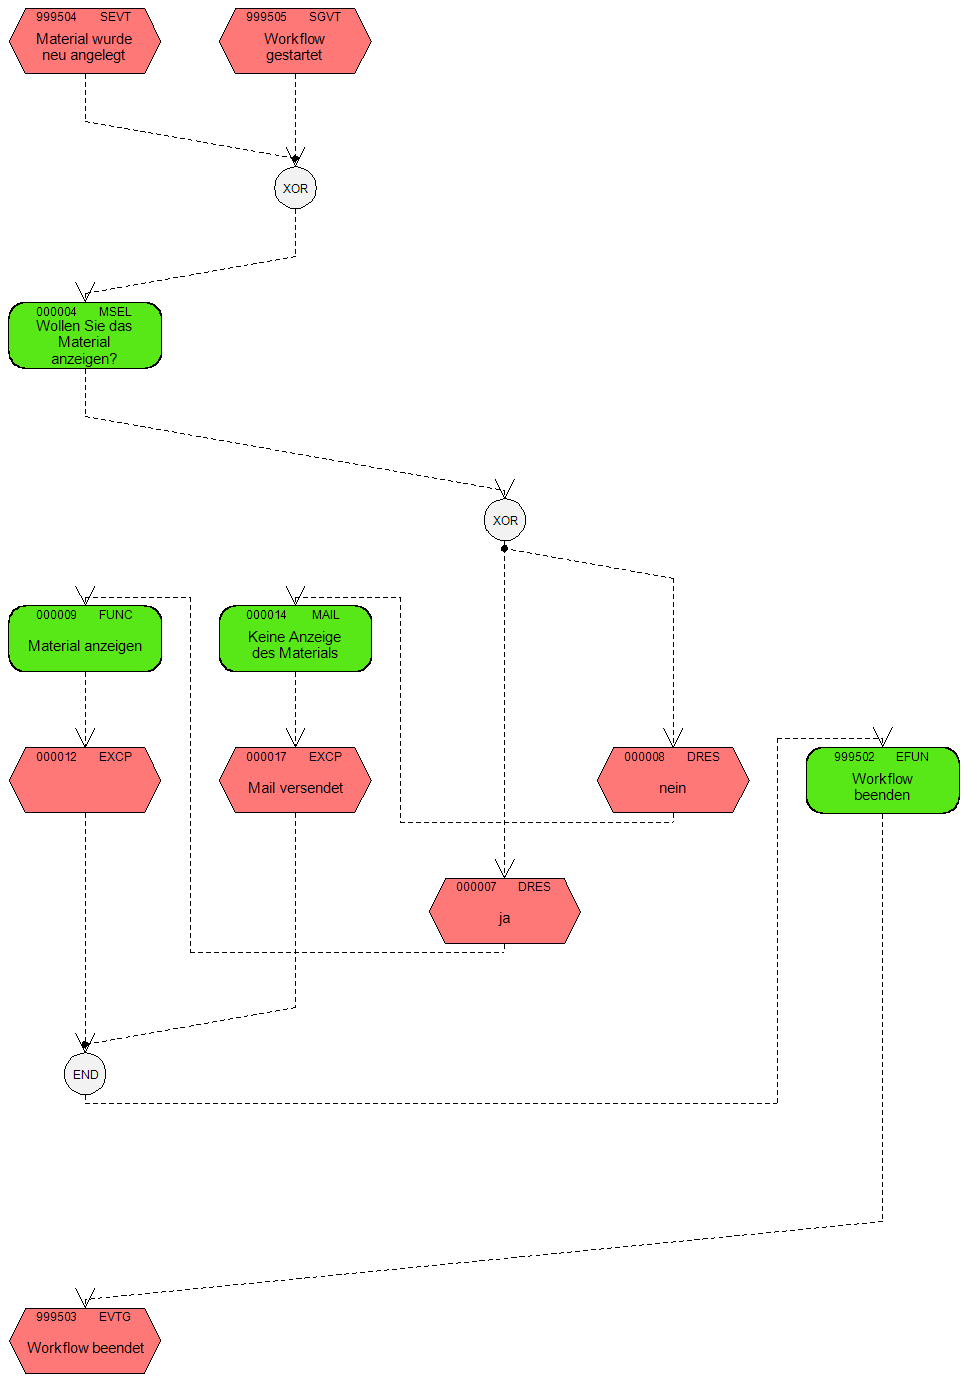
\includegraphics[height=0.9\textheight]{grafiken/wf-builder_view-classicepc.png}
	\caption{Ansicht eines Workflows als klassisches EPK}
	\vspace{-10pt}
	\label{abb:workflow-view-classicepc}
	\end{center}
\end{figure}

\begin{figure}[H]
	\begin{center}
	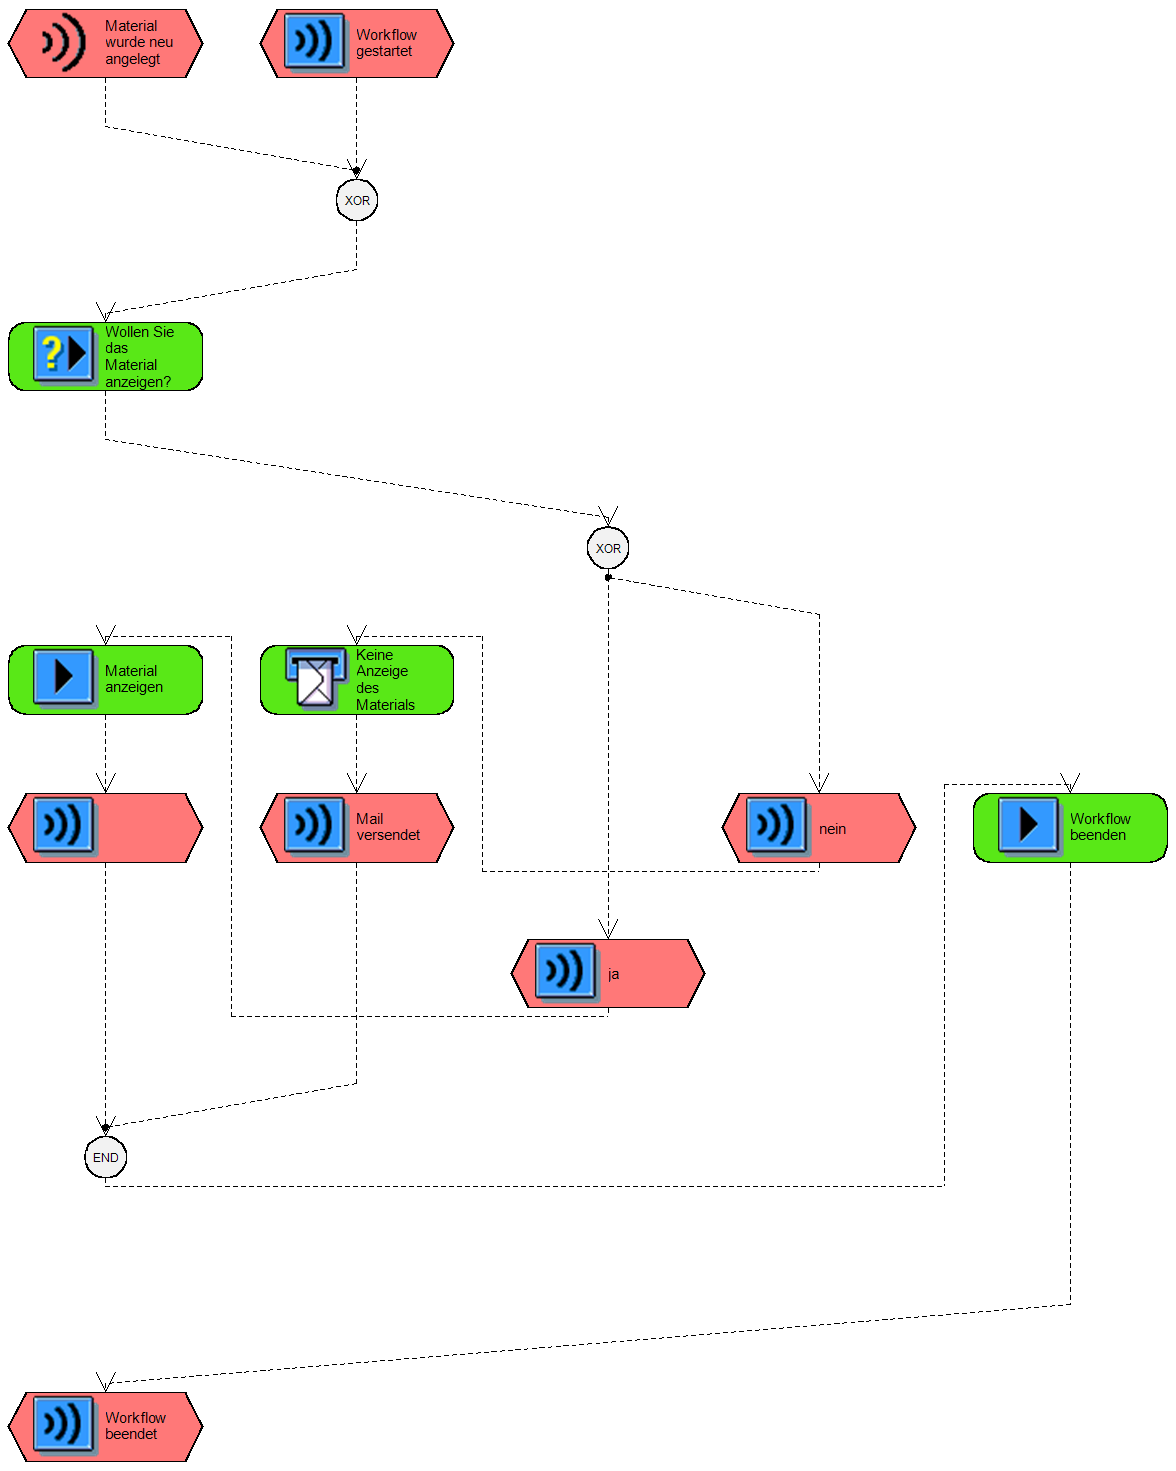
\includegraphics[width=1.0\textwidth]{grafiken/wf-builder_view-epc.png}
	\caption{Ansicht eines Workflows als Mischform beider Ansichten}
	\vspace{-10pt}
	\label{abb:workflow-view-epc}
	\end{center}
\end{figure}

\begin{figure}[H]
	\begin{center}
	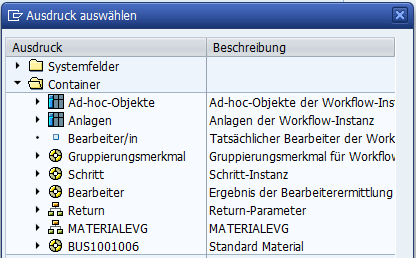
\includegraphics[width=250px]{grafiken/wf-builder_bsp1_formular-aufgabe_eingabehilfe-ausdruck.png}
	\caption{Eingabehilfe zum Ausdruck bei neuen Aufgaben}
	\vspace{-10pt}
	\label{abb:workflow-bsp1-aufgaben_form-inputhelp}
	\end{center}
\end{figure}

\begin{figure}[H]
	\begin{center}
	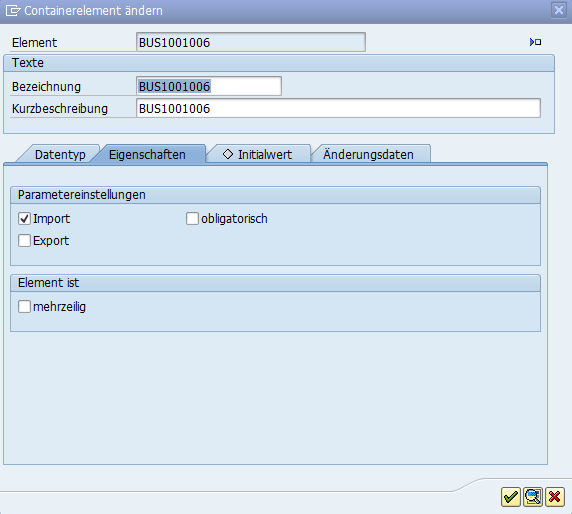
\includegraphics[width=350px]{grafiken/wf-builder_bsp1_formular-containerelement-edit.png}
	\caption{Einstellung zum Import eines Containerelements}
	\vspace{-10pt}
	\label{abb:workflow-bsp1-containeredit-import}
	\end{center}
\end{figure}

\begin{figure}[H]
	\begin{center}
	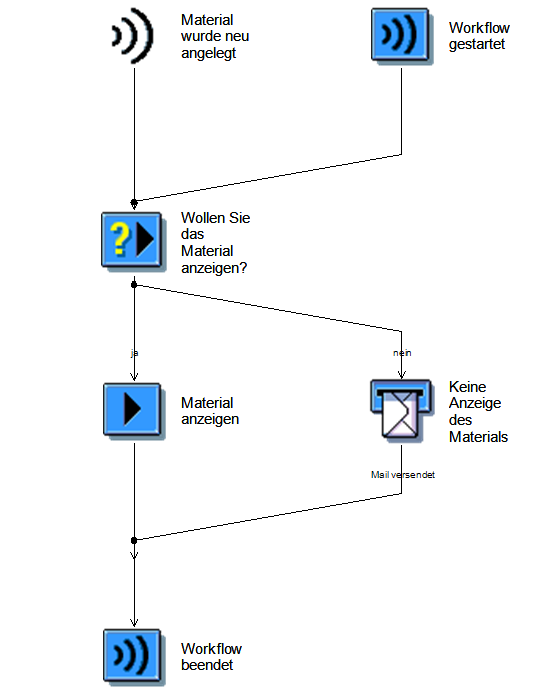
\includegraphics[height=0.7\textheight]{grafiken/wf-builder_bsp1_complete.png}
	\caption{Erster Beispielworkflow fertiggestellt}
	\vspace{-10pt}
	\label{abb:workflow-bsp1-complete}
	\end{center}
\end{figure}

\begin{figure}[H]
	\begin{center}
	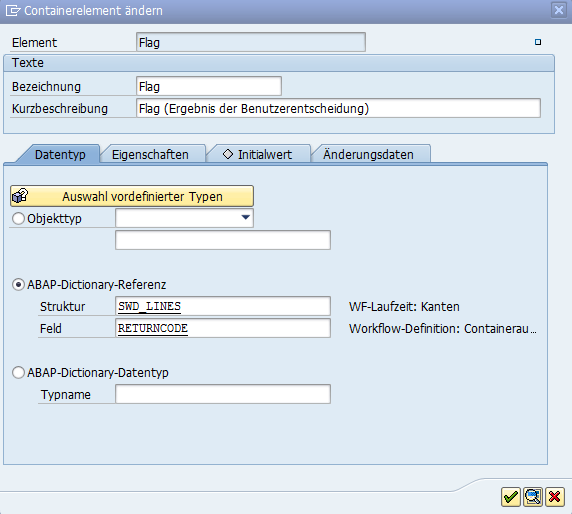
\includegraphics[height=400px]{grafiken/wf-builder_bsp2_container-flag.png}
	\caption{Konfiguration eines Containerelements als Flag}
	\vspace{-10pt}
	\label{abb:workflow-bsp2-container-flag}
	\end{center}
\end{figure}

\begin{figure}[H]
	\begin{center}
	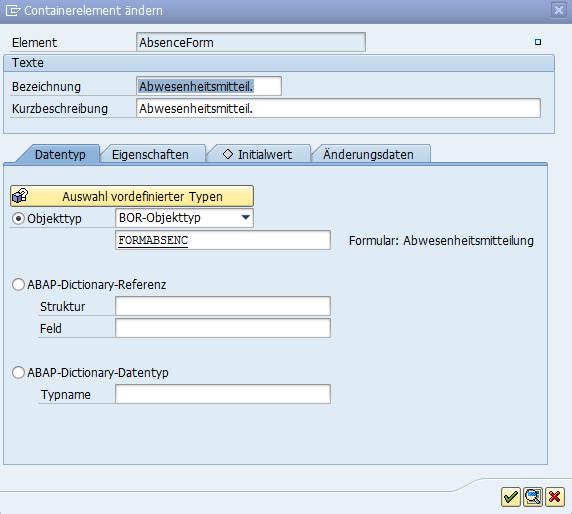
\includegraphics[height=400px]{grafiken/wf-builder_bsp2_container-form.png}
	\caption{Konfiguration eines Containerelements als Formular zur Abwesenheitsmitteilung}
	\vspace{-10pt}
	\label{abb:workflow-bsp2-container-form}
	\end{center}
\end{figure}

\begin{figure}[H]
	\begin{center}
	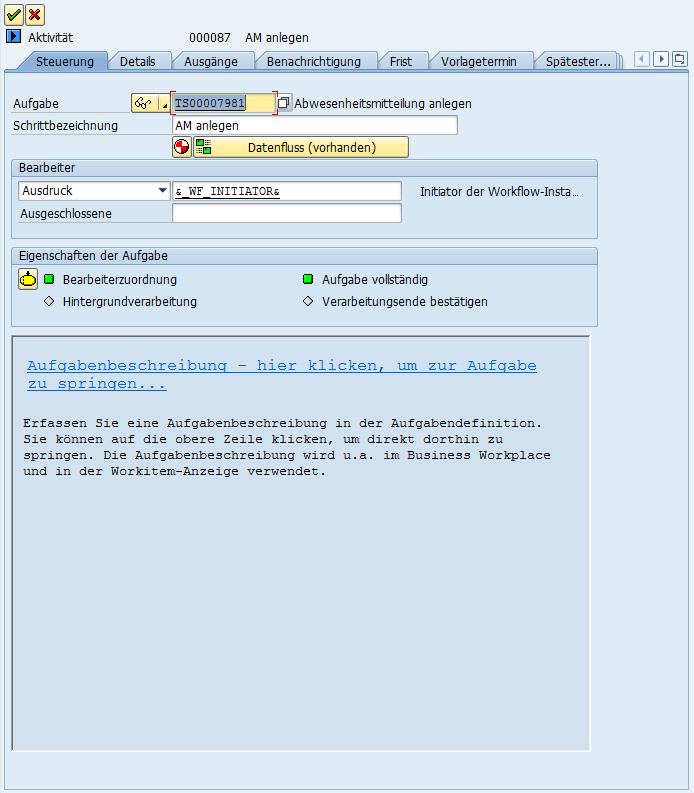
\includegraphics[width=1.0\textwidth]{grafiken/wf-builder_bsp2_act_am-anlegen.png}
	\caption{Konfiguration der Aufgabe Abwesenheitsmitteilung anlegen}
	\vspace{-10pt}
	\label{abb:workflow-bsp2-act_am-anlegen}
	\end{center}
\end{figure}

\begin{figure}[H]
	\begin{center}
	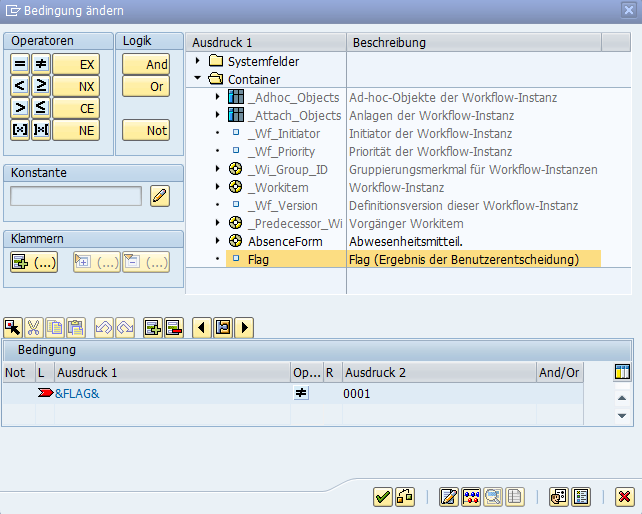
\includegraphics[width=450px]{grafiken/wf-builder_bsp2_act_loop_inputhelp.png}
	\caption{Eingabehilfe der Until-Schleife}
	\vspace{-10pt}
	\label{abb:workflow-bsp2-act_loop_inputhelp}
	\end{center}
\end{figure}

\begin{figure}[H]
	\begin{center}
	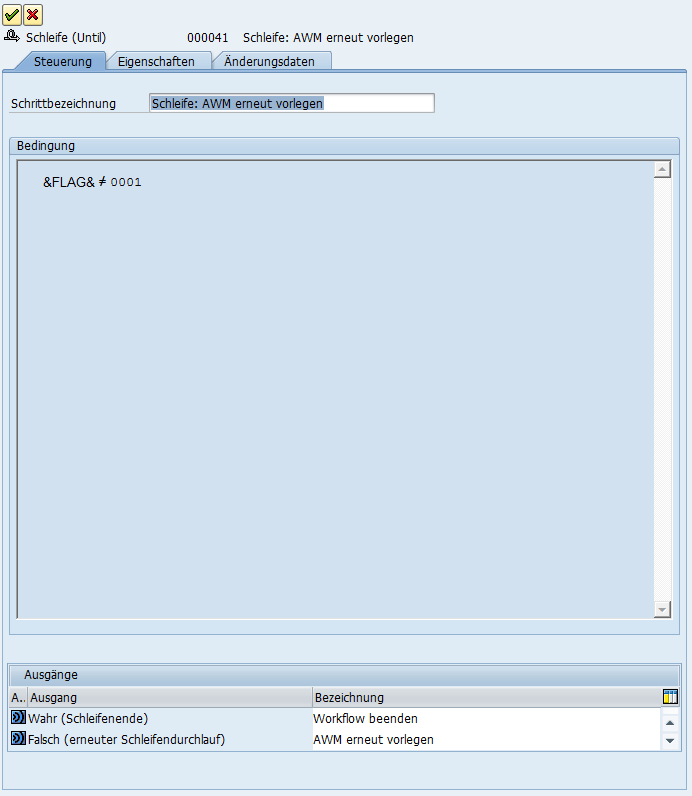
\includegraphics[width=1.0\textwidth]{grafiken/wf-builder_bsp2_act_loop.png}
	\caption{Konfiguration der Until-Schleife}
	\vspace{-10pt}
	\label{abb:workflow-bsp2-act_loop}
	\end{center}
\end{figure}

\begin{figure}[H]
	\begin{center}
	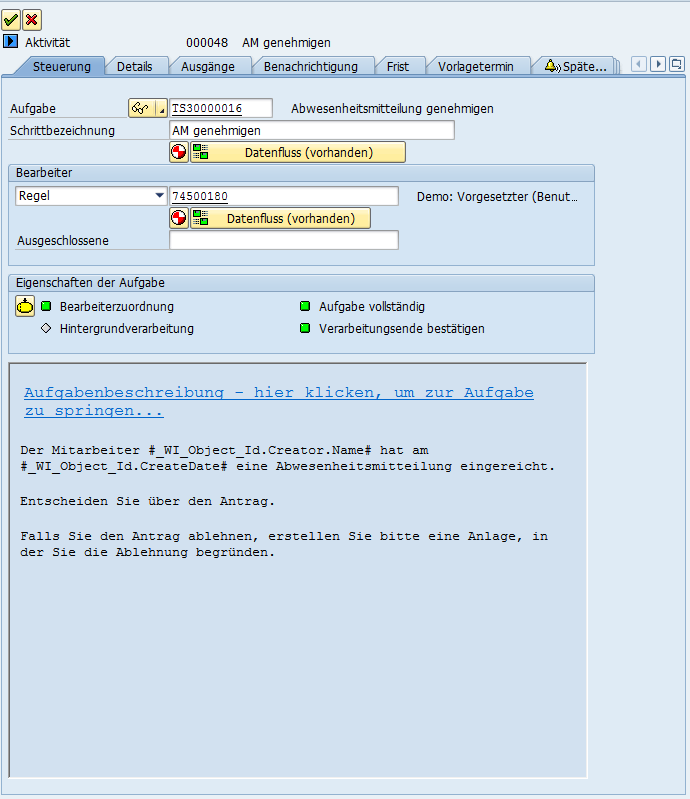
\includegraphics[width=1.0\textwidth]{grafiken/wf-builder_bsp2_act_am-genehmigen.png}
	\caption{Konfiguration der Aufgabe Abwesenheitsmitteilung genehmigen}
	\vspace{-10pt}
	\label{abb:workflow-bsp2-act_am-genehmigen}
	\end{center}
\end{figure}

\begin{figure}[H]
	\begin{center}
	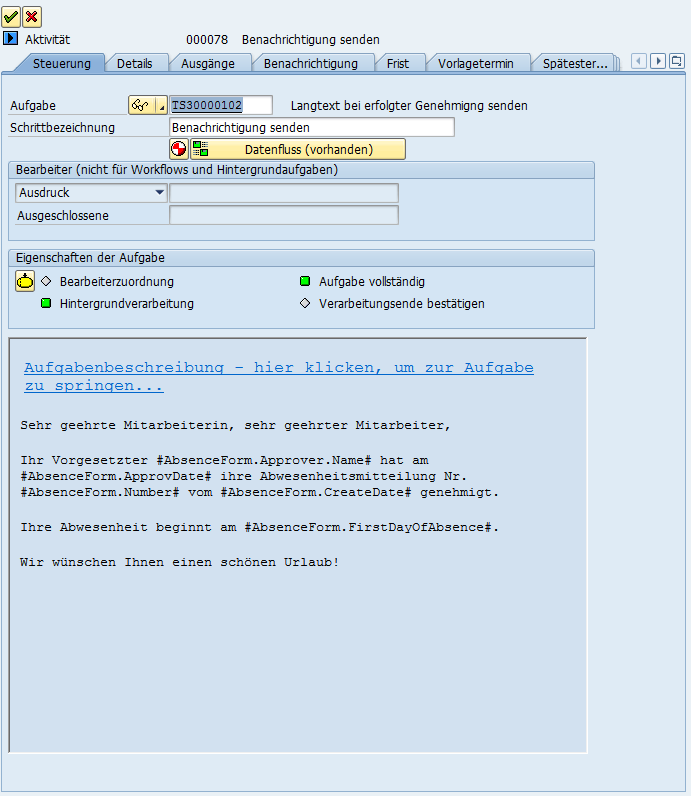
\includegraphics[width=1.0\textwidth]{grafiken/wf-builder_bsp2_act_message-genehmigt.png}
	\caption{Konfiguration der Aufgabe Benachrichtigung über Genehmigung}
	\vspace{-10pt}
	\label{abb:workflow-bsp2-act_message-genehmigt}
	\end{center}
\end{figure}

\begin{figure}[H]
	\begin{center}
	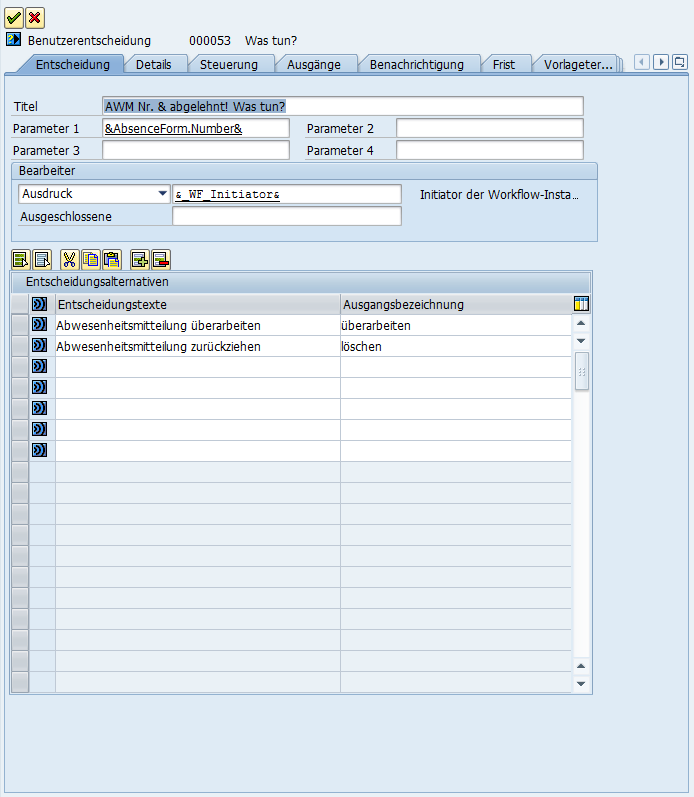
\includegraphics[width=1.0\textwidth]{grafiken/wf-builder_bsp2_act_was-tun.png}
	\caption{Konfiguration der Benutzerentscheidung nach Ablehnung}
	\vspace{-10pt}
	\label{abb:workflow-bsp2-act_was-tun}
	\end{center}
\end{figure}

\begin{figure}[H]
	\begin{center}
	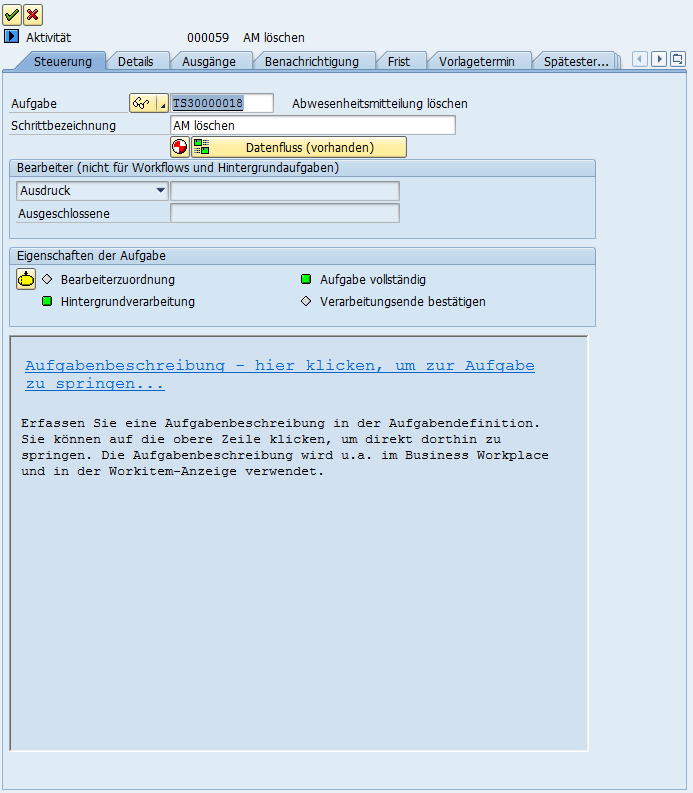
\includegraphics[width=1.0\textwidth]{grafiken/wf-builder_bsp2_act_am-loeschen.png}
	\caption{Konfiguration der Aufgabe zum Löschen einer Abwesenheitsmitteilung}
	\vspace{-10pt}
	\label{abb:workflow-bsp2-act_am-loeschen}
	\end{center}
\end{figure}

\begin{figure}[H]
	\begin{center}
	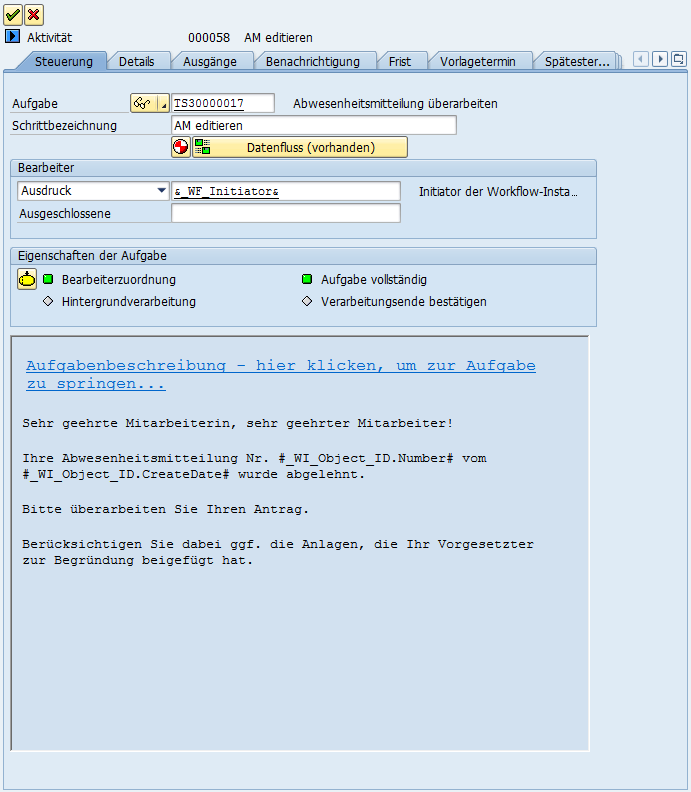
\includegraphics[width=1.0\textwidth]{grafiken/wf-builder_bsp2_act_am-editieren.png}
	\caption{Konfiguration der Aufgabe zum Editieren einer Abwesenheitsmitteilung}
	\vspace{-10pt}
	\label{abb:workflow-bsp2-act_am-editieren}
	\end{center}
\end{figure}

\begin{figure}[H]
	\begin{center}
	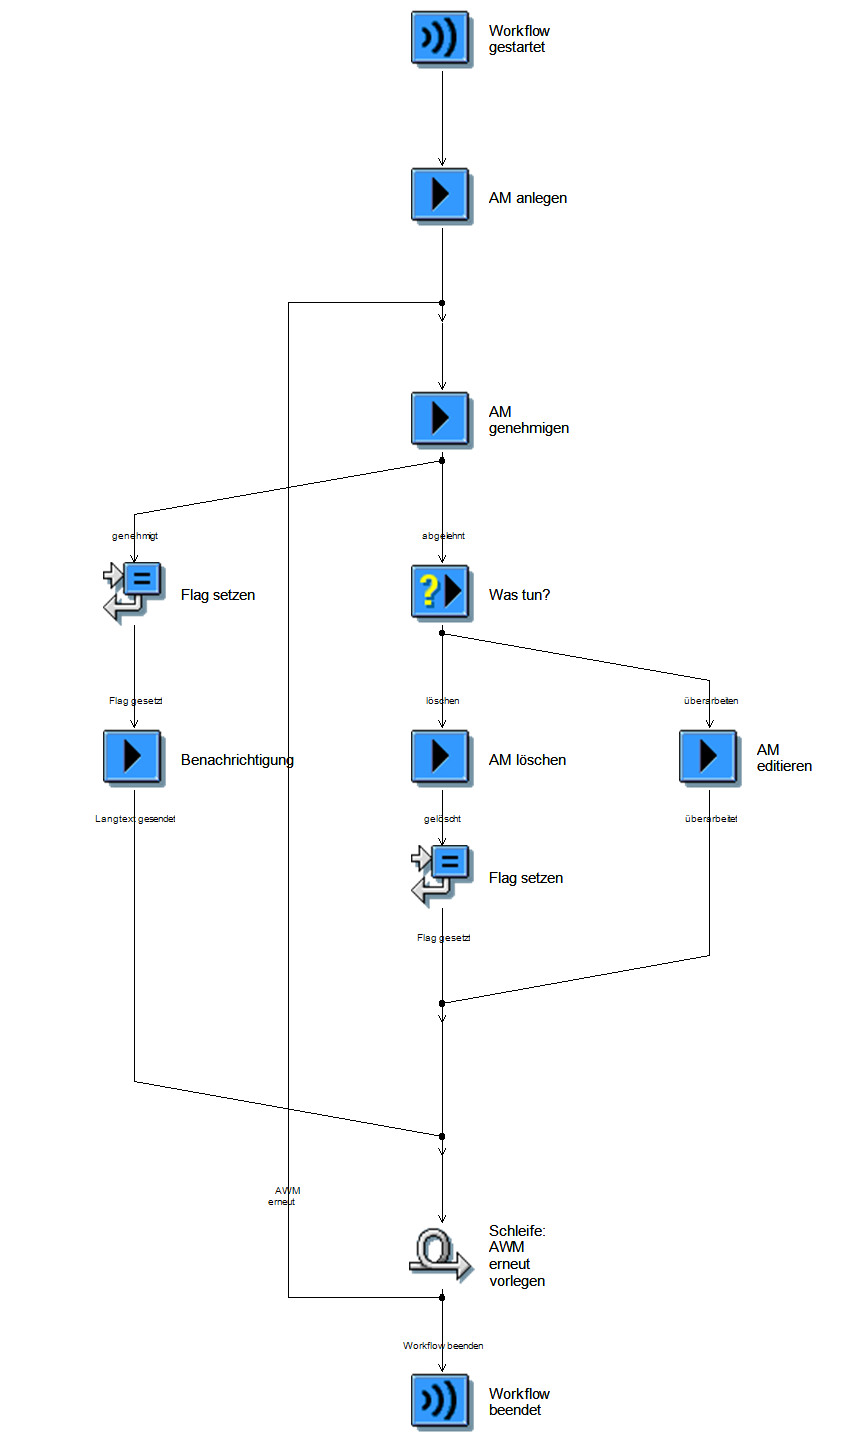
\includegraphics[height=0.95\textheight]{grafiken/wf-builder_bsp2_complete.png}
	\caption{Zweiter Beispielworkflow fertiggestellt}
	\vspace{-10pt}
	\label{abb:workflow-bsp2-complete}
	\end{center}
\end{figure}

\section{Business ByDesign Screenshots}

\begin{figure}[H]
	\begin{center}
	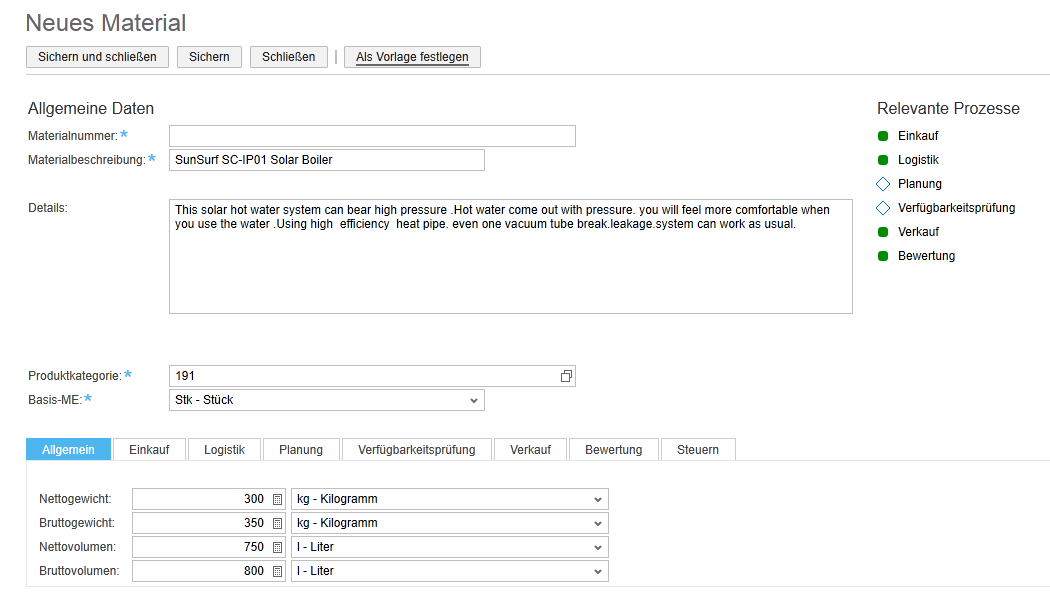
\includegraphics[width=1.0\textwidth]{grafiken/ByDesign-HowTo-1.png}
	\caption{Neues Material anlegen}
	\vspace{-10pt}
	\label{abb:byd-newmaterial}
	\end{center}
\end{figure}

\begin{figure}[H]
	\begin{center}
	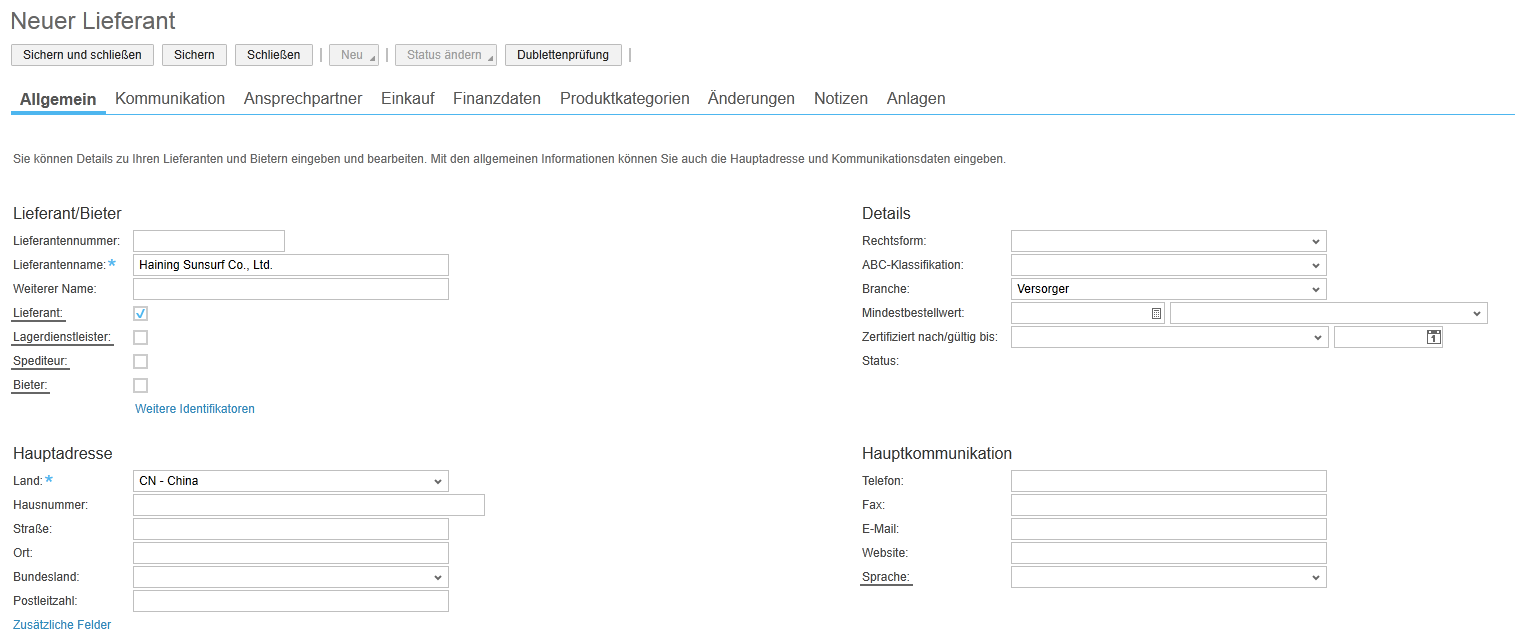
\includegraphics[width=1.0\textwidth]{grafiken/ByDesign-HowTo-2.png}
	\caption{Neuen Zulieferer anlegen}
	\vspace{-10pt}
	\label{abb:byd-newsupplier}
	\end{center}
\end{figure}

\begin{figure}[H]
	\begin{center}
	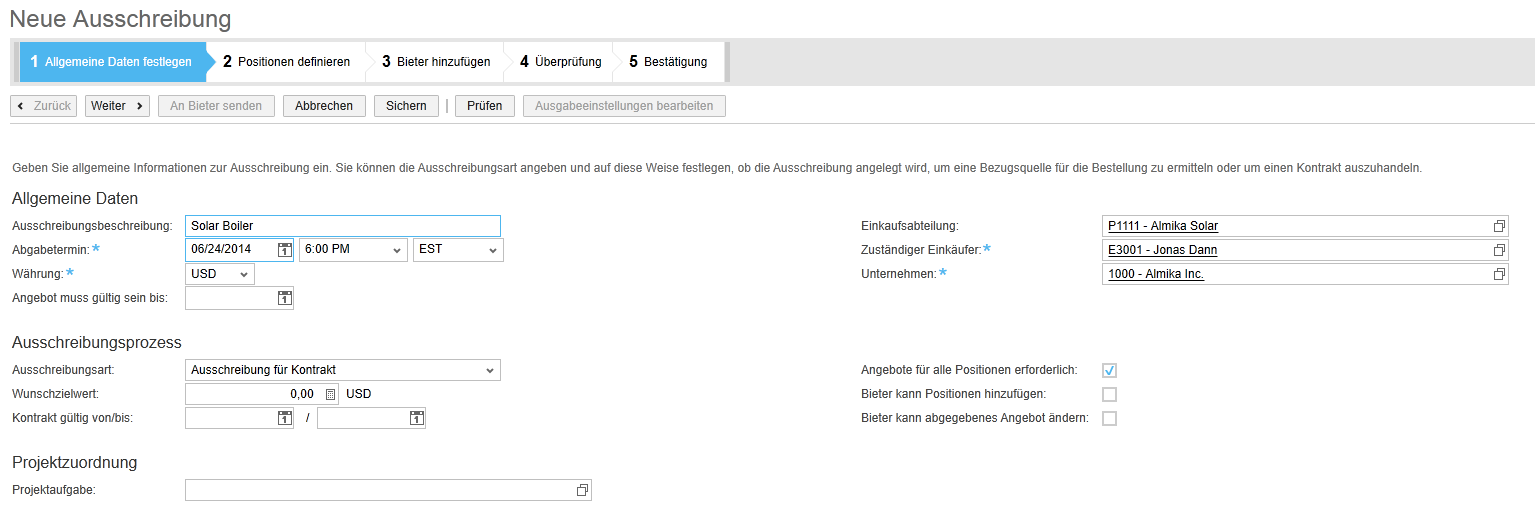
\includegraphics[width=1.0\textwidth]{grafiken/ByDesign-HowTo-Ausschreibung-1.png}
	\caption{Neue Ausschreibung erstellen - Allgemeine Daten}
	\vspace{-10pt}
	\label{abb:byd-rfq-1}
	\end{center}
\end{figure}

\begin{figure}[H]
	\begin{center}
	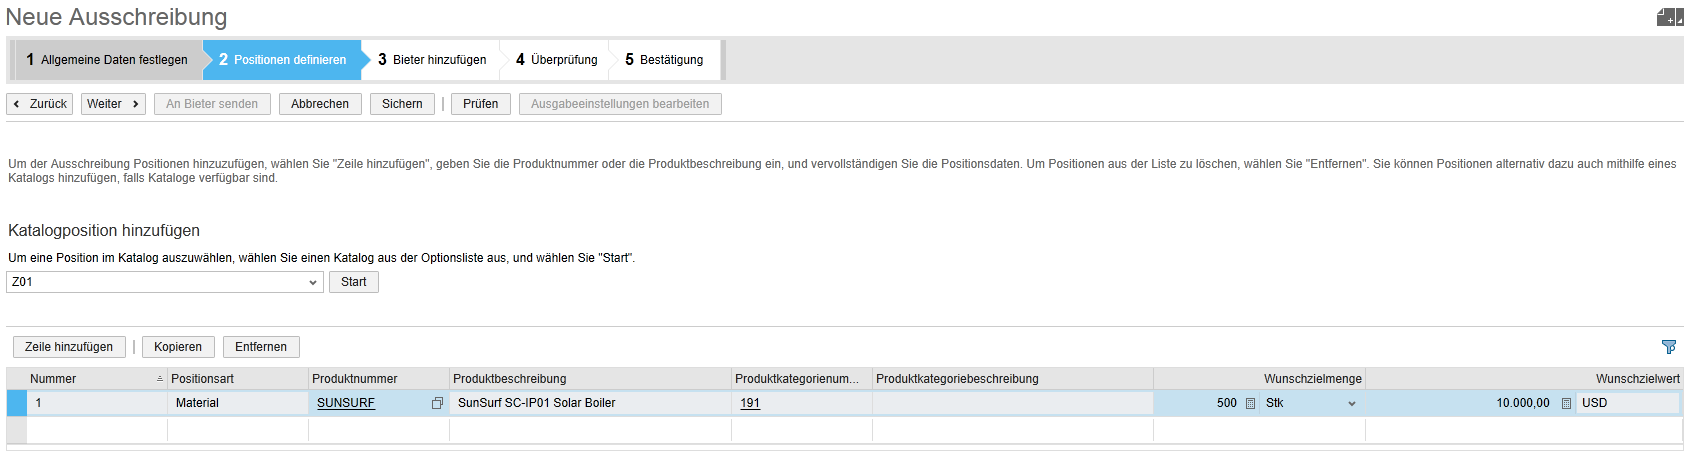
\includegraphics[width=1.0\textwidth]{grafiken/ByDesign-HowTo-Ausschreibung-2.png}
	\caption{Neue Ausschreibung erstellen - Positionen definieren}
	\vspace{-10pt}
	\label{abb:byd-rfq-2}
	\end{center}
\end{figure}

\begin{figure}[H]
	\begin{center}
	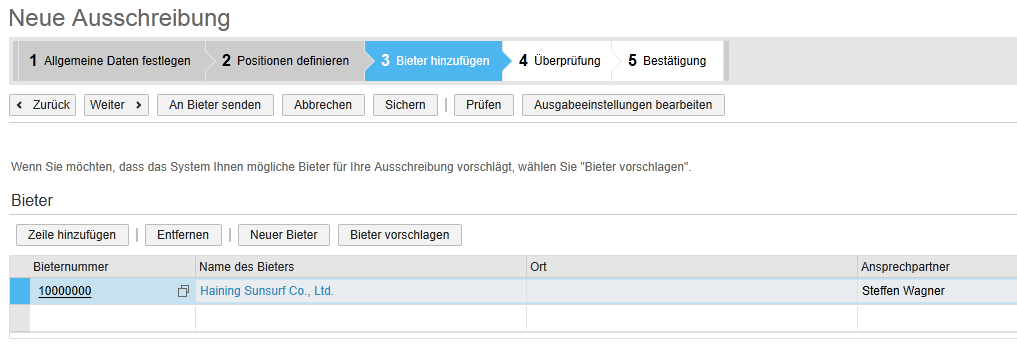
\includegraphics[width=1.0\textwidth]{grafiken/ByDesign-HowTo-Ausschreibung-3.png}
	\caption{Neue Ausschreibung erstellen - Bieter hinzufügen}
	\vspace{-10pt}
	\label{abb:byd-rfq-3}
	\end{center}
\end{figure}

\begin{figure}[H]
	\begin{center}
	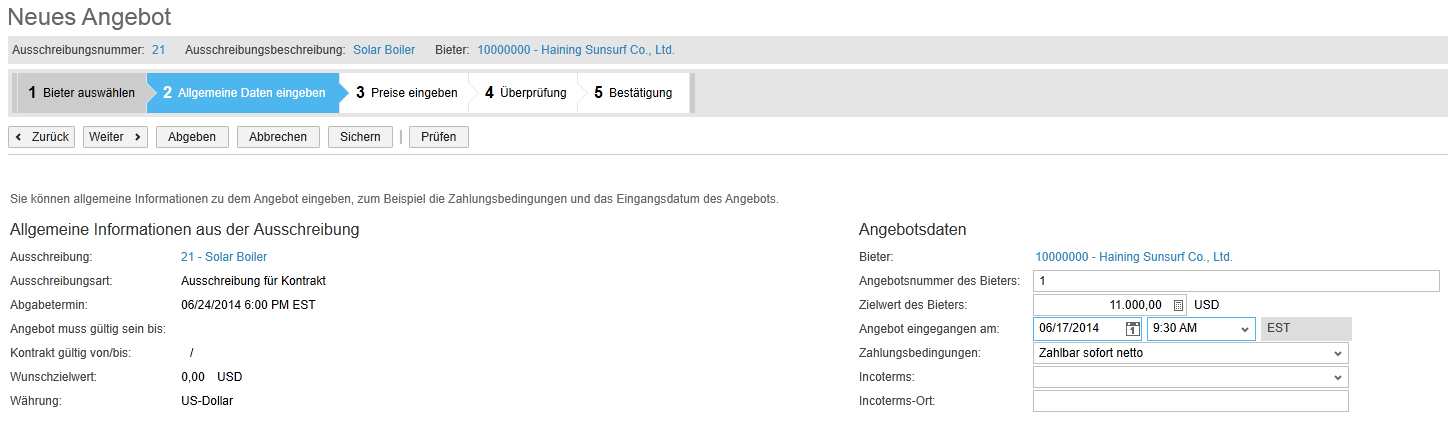
\includegraphics[width=1.0\textwidth]{grafiken/ByDesign-HowTo-Ausschreibung-4.png}
	\caption{Neues Angebot - Allgemeine Daten}
	\vspace{-10pt}
	\label{abb:byd-rfq-4}
	\end{center}
\end{figure}

\begin{figure}[H]
	\begin{center}
	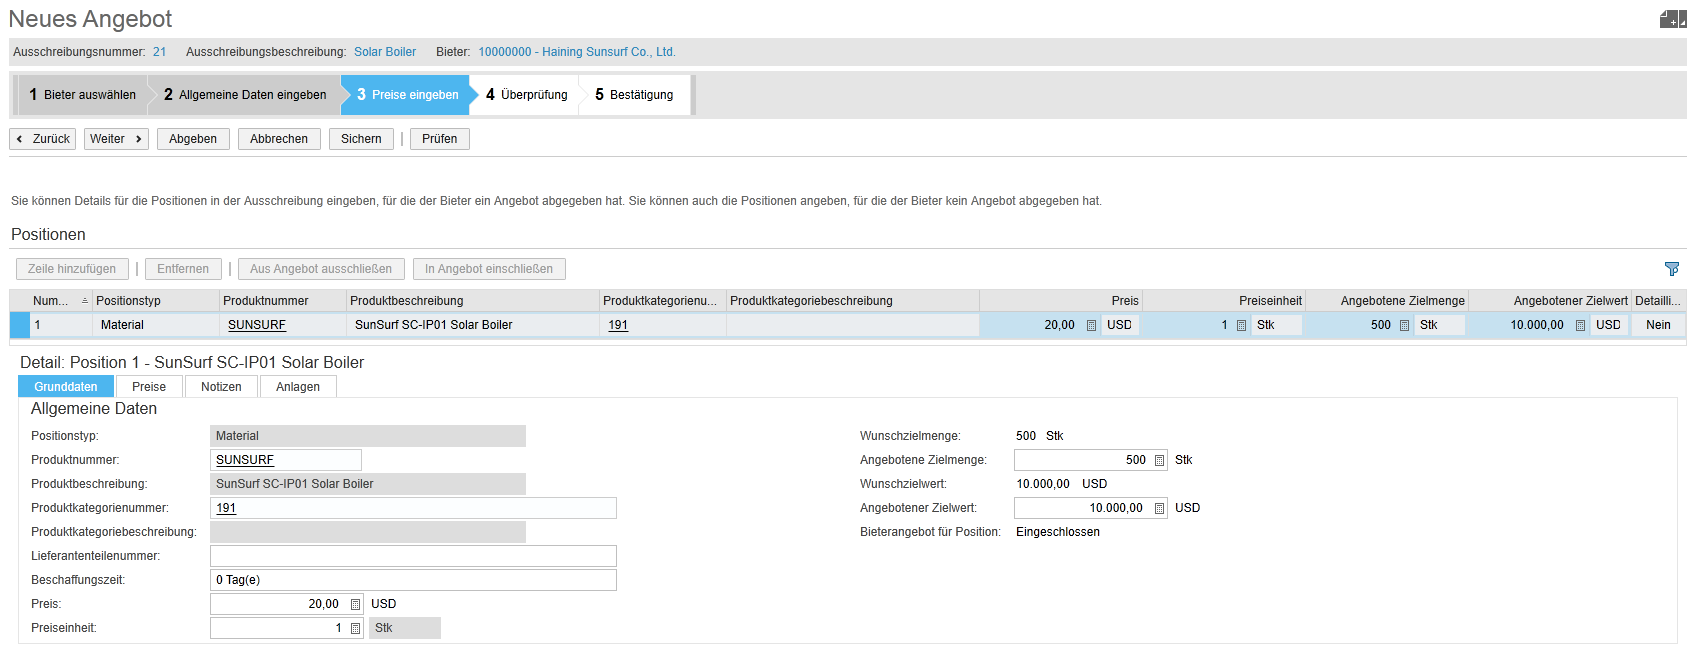
\includegraphics[width=1.0\textwidth]{grafiken/ByDesign-HowTo-Ausschreibung-5.png}
	\caption{Neues Angebot - Preise einfügen}
	\vspace{-10pt}
	\label{abb:byd-rfq-5}
	\end{center}
\end{figure}

\begin{figure}[H]
	\begin{center}
	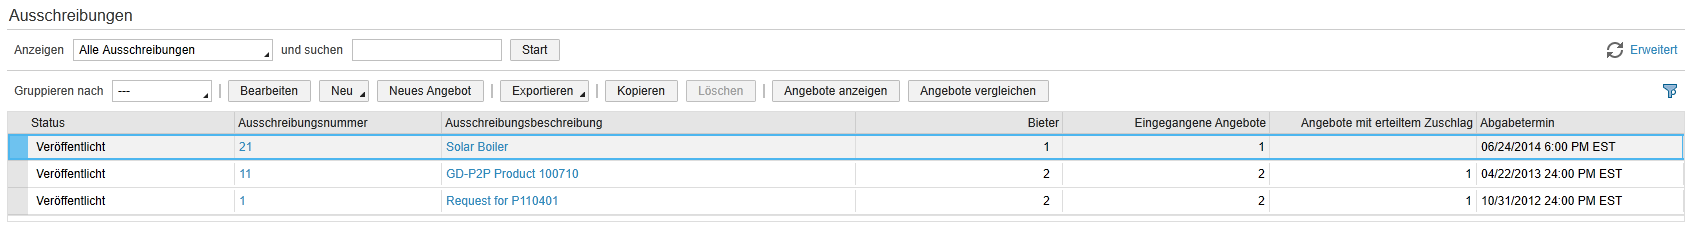
\includegraphics[width=1.0\textwidth]{grafiken/ByDesign-HowTo-Ausschreibung-6.png}
	\caption{Übersicht: Ausschreibungen}
	\vspace{-10pt}
	\label{abb:byd-rfq-6}
	\end{center}
\end{figure}

\begin{figure}[H]
	\begin{center}
	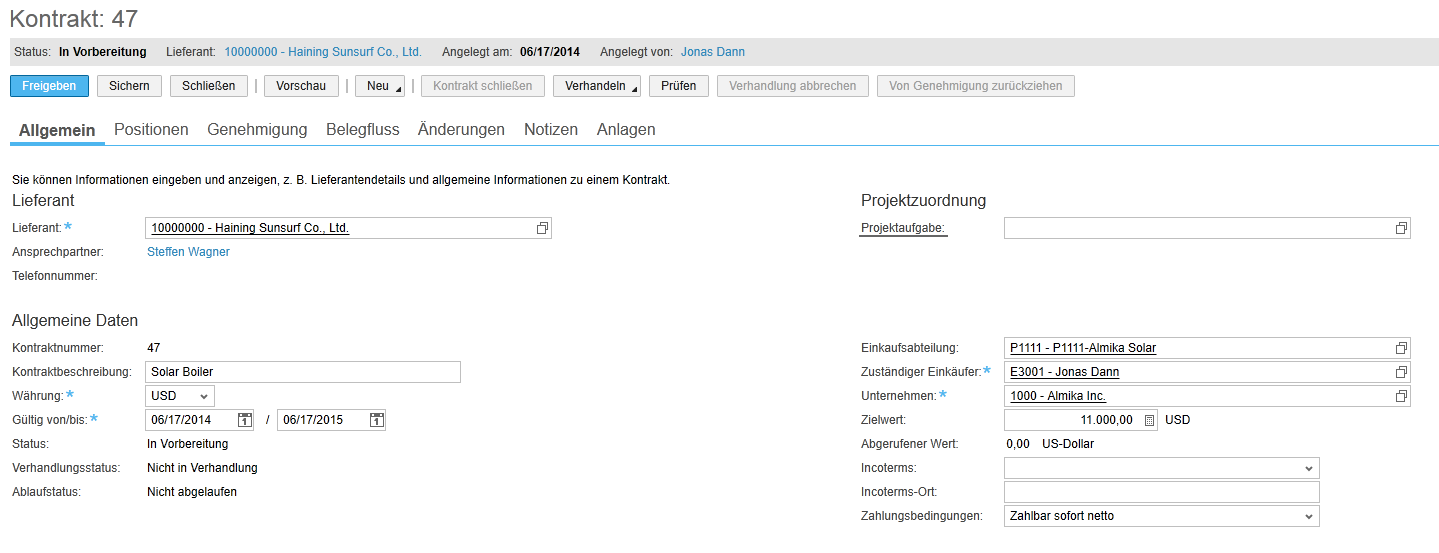
\includegraphics[width=1.0\textwidth]{grafiken/ByDesign-HowTo-4.png}
	\caption{Vertrag schließen}
	\vspace{-10pt}
	\label{abb:byd-contract}
	\end{center}
\end{figure}

\vspace{-10pt}

%GLOSSARIES
\printglossary[type=\acronymtype]
%%% \newpage just to demonstrate that links are correct
\newpage
\printglossary[type=main]

% manchmal muss man etwas tricksen, damit alles auf 1 Seite passt:
% ("vertical space" mit negativem Abstand)
\vspace{-1.0cm}

%% zum guten Schluss kommt das Literaturverzeichnis
% Darstellungsart festlegen:
% http://www.cs.stir.ac.uk/~kjt/software/latex/showbst.html
\bibliographystyle{acm}

% Datei meineliteratur.bib einbinden.
\bibliography{includes/meineliteratur}

% Selbstständigkeitserklärung
\thispagestyle{empty}
\section*{Selbstständigkeitserklärung}
\vspace{15mm}
 
Der Verfasser erklärt, dass er die vorliegende Arbeit selbständig, 
ohne fremde Hilfe und ohne Benutzung anderer als der angegebenen Hilfsmittel
angefertigt hat. 
Die aus fremden Quellen (einschließlich elektronischer Quellen) direkt oder 
indirekt übernommenen Gedanken sind ausnahmslos als solche kenntlich gemacht. 
 
%% Abstand und Linie
% 3 Spalten (für alle 3 Leute)
\vspace{3cm} 
Walldorf, den \today
\vspace{1cm} 	
\begin{multicols}{3}
	\vspace{2cm}
	\rule{5cm}{.1pt}\\
	\vspace{5mm}
	Steffen Wagner
	
	\rule{5cm}{.1pt}\\
	\vspace{5mm}
	Jonas Dann

	\rule{5cm}{.1pt}\\
	\vspace{5mm}
	Marco Dörfler
\end{multicols}

\vspace{5cm}

%%%%%
\end{document}
%%%%%